\documentclass{beamer}
%\usetheme{Berkeley}
\usetheme{Singapore}
%\setbeamercolor{structure}{fg=blue}
\usepackage{upgreek}
\usepackage{color}
%\def\magyarOptions{hyphenation=huhyphn}
%\usepackage{ae,aecompl}
%\usepackage[T1]{fontenc}
\usepackage[utf8]{inputenc}
%\usepackage[hungarian]{babel}
\usepackage{gensymb}
\usepackage{tikz}
\usepackage[framemethod=tikz]{mdframed}
\normalfont
\title{Recent Advances in Potentiometric Scanning Electrochemical Microscopy}
\author
{author:\\
András Kiss\\
\hfill \\
supervisor:\\
prof. Géza Nagy}

\institute
{
  %\inst{1}%
  Department of General and Physical Chemistry\\
  University of Pécs, Hungary\\
  \hfill \\

  
\includegraphics[width=0.14\textwidth]{pte_logo.eps}\\
  April 18, 2017
}

\date[]

\begin{document}
\frame{\titlepage}  


\begin{frame}
	\centering
	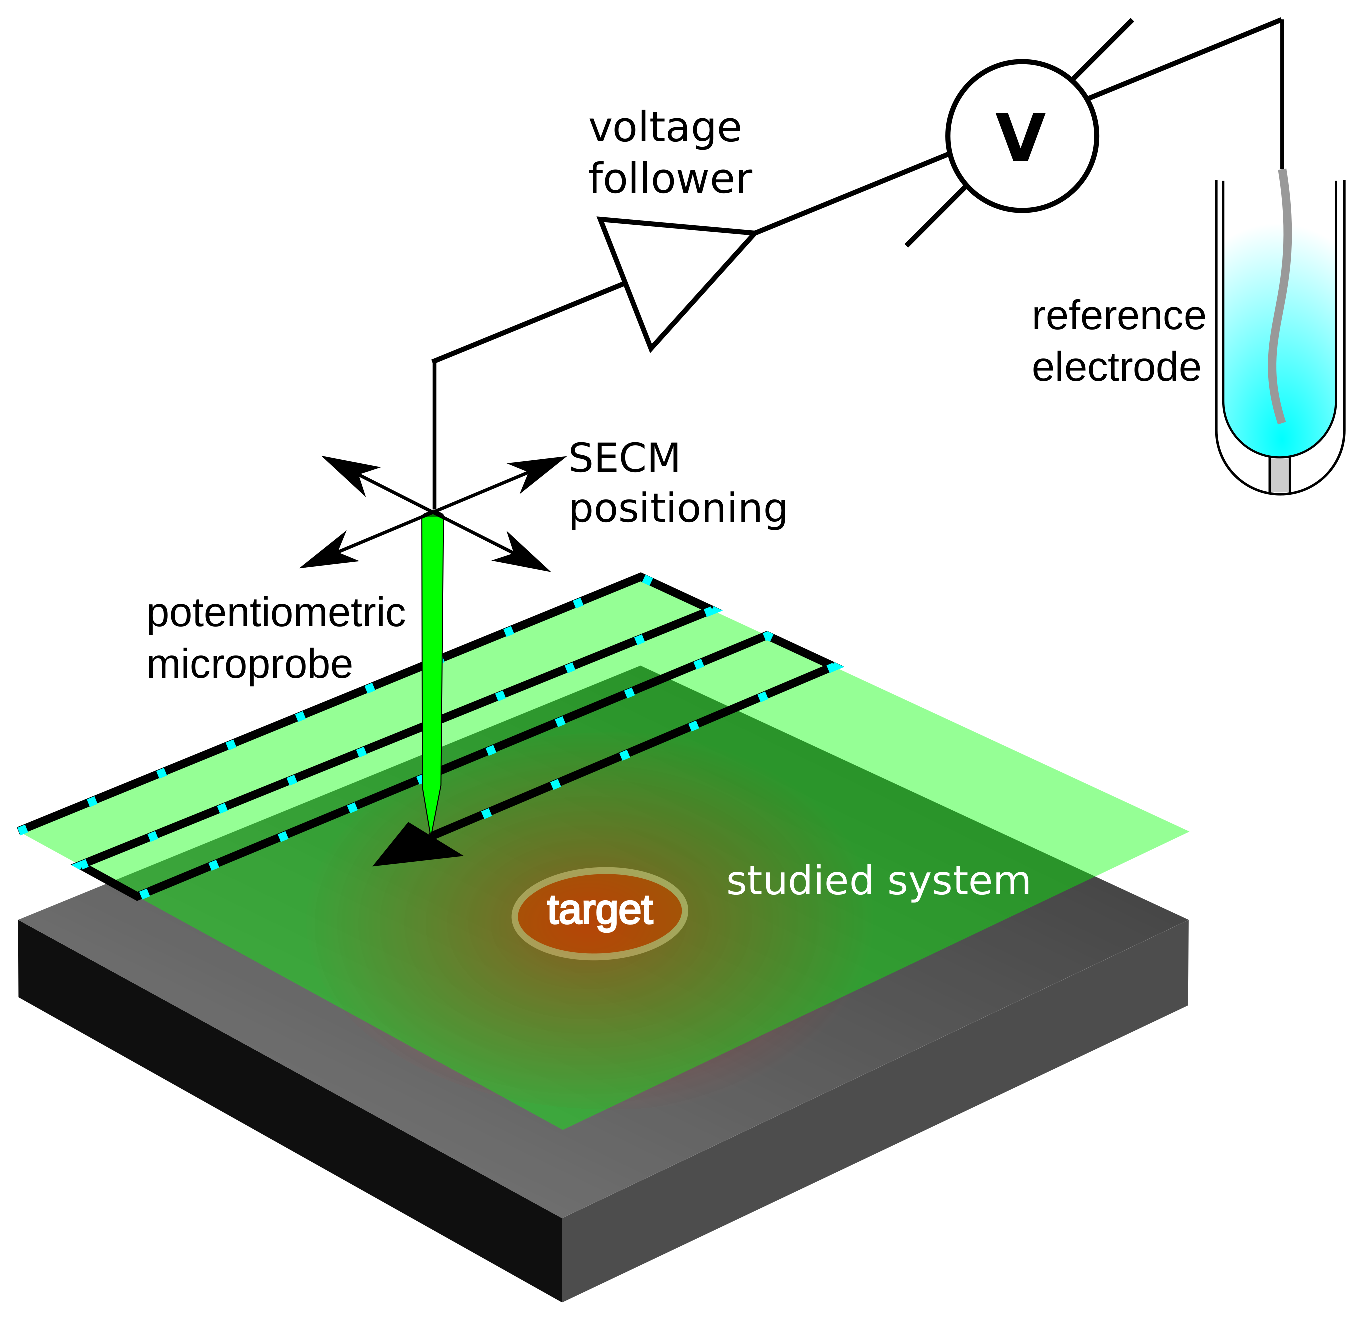
\includegraphics[width=0.6\textwidth]{secm.eps}
	\frametitle{Potentiometric Scanning Electrochemical Microscopy}
	\framesubtitle{A Scanning Probe Microscopic technique}

\end{frame}


\begin{frame}
\frametitle{Ion-selective micropipettes}
\framesubtitle{As SECM probes}
\begin{columns}[T] % align columns
\begin{column}{.48\textwidth}

\centering
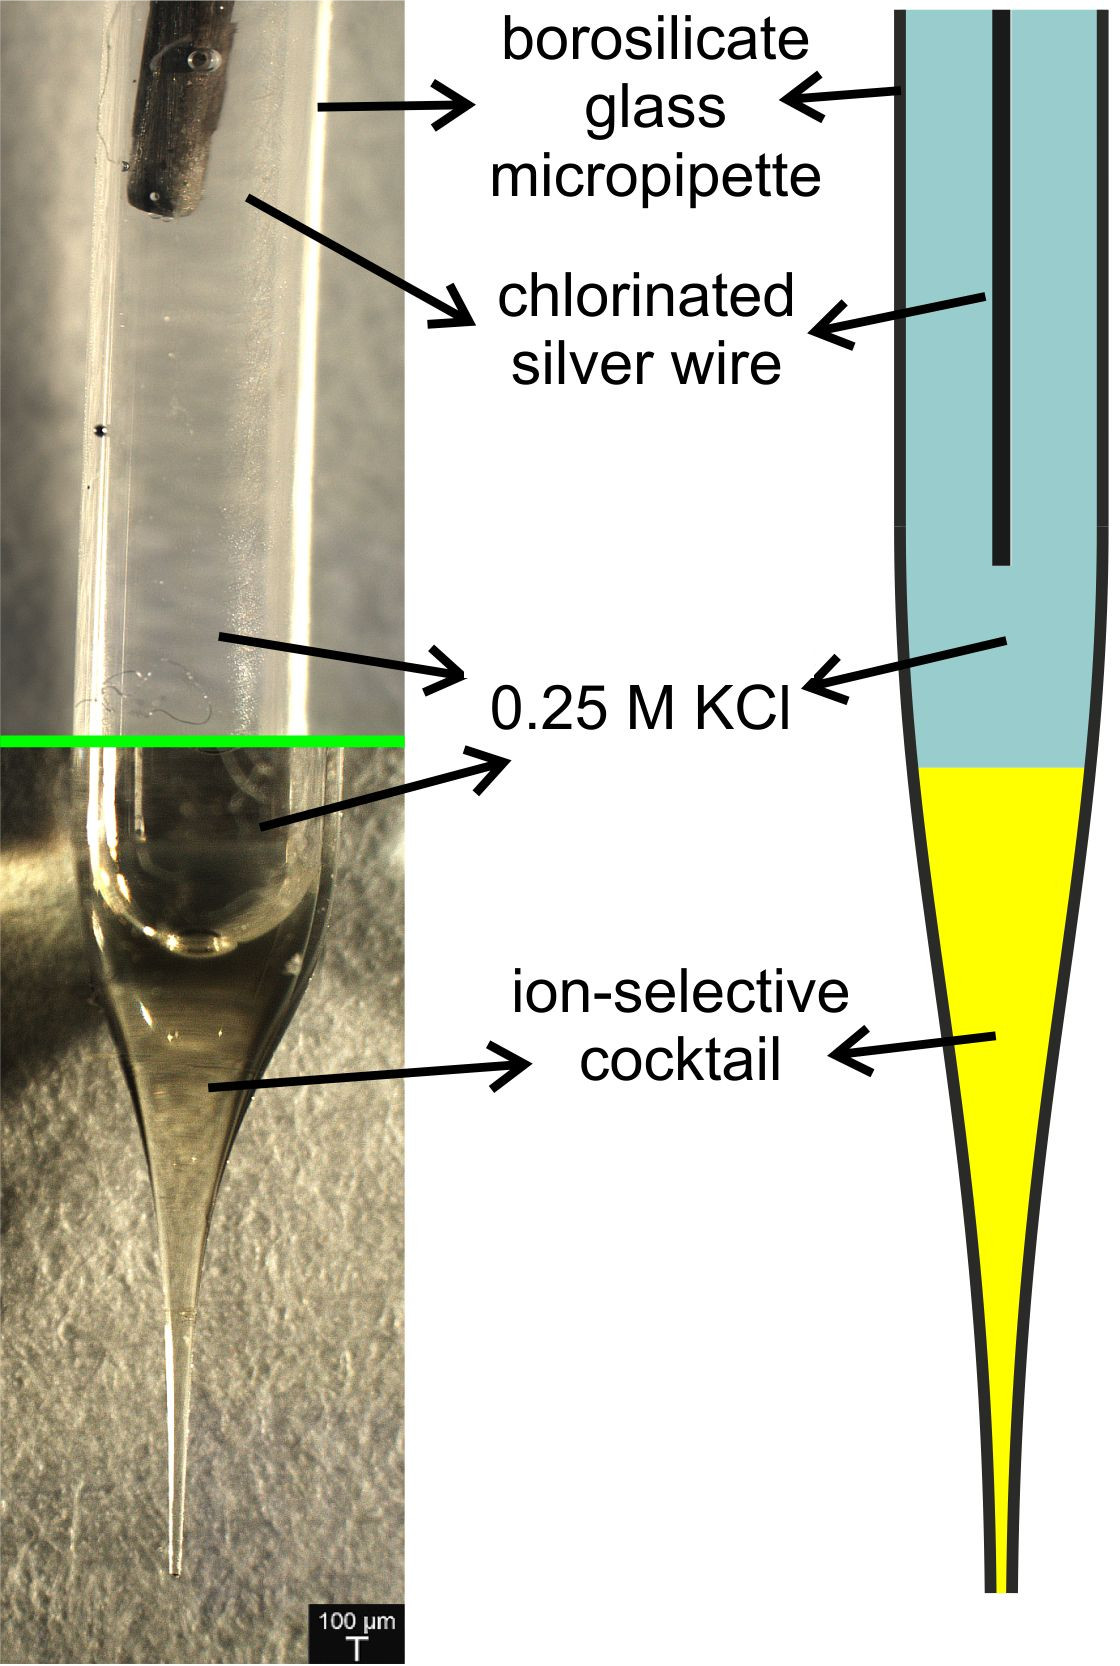
\includegraphics[width=0.9\textwidth]{liquid.jpg}
\end{column}%
\hfill%
\begin{column}{.48\textwidth}
%\color{blue}\rule{\linewidth}{4pt}
\centering

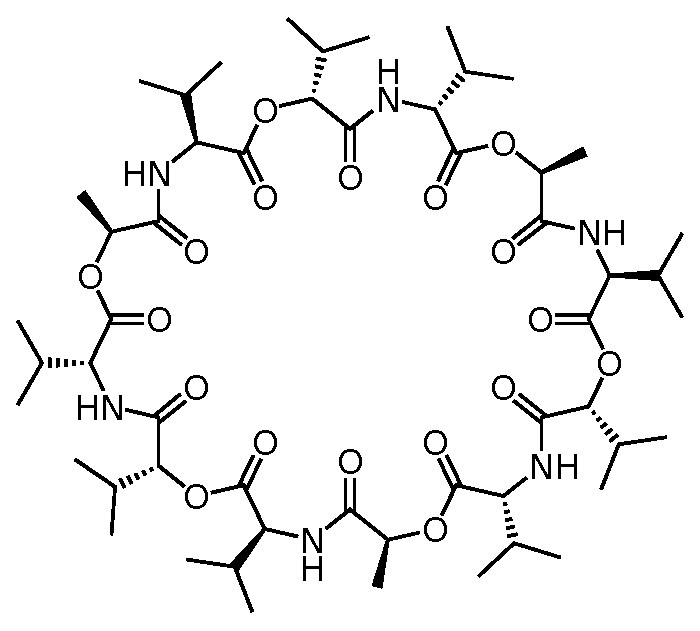
\includegraphics[width=0.8\textwidth]{Valinomycin.eps}

Valinomycin
\vfill

\footnotesize
\begin{equation*}
        E=E^\theta + \frac{RT}{z_iF} \ln \left [ a_i + \sum_{j} \left ( k_{ij}a_j^{z_i/z_j} \right ) \right ]
        \end{equation*}
\normalsize
Nikolsky--equation
\end{column}%
\end{columns}
\end{frame}

\begin{frame}
	\frametitle{The problem with potentiometric SECM} 
	\framesubtitle{Distortion at high scan rate}
	\centering
	\includegraphics[trim = 10mm 30mm 0mm 20mm, clip, width=0.4\textwidth, angle=-90]{real.eps}\hfill\includegraphics[trim = 10mm 30mm 0mm 20mm, clip, width=0.4\textwidth, angle=-90]{fastcomb_sim.eps}
\end{frame}

\begin{frame}
	\frametitle{Why is the image distorted?}
	\framesubtitle{The RC time constant} 
	\centering
	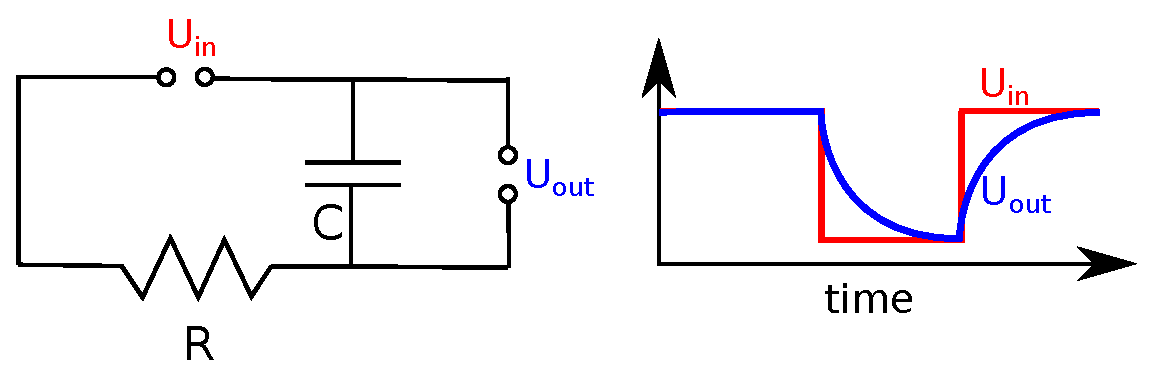
\includegraphics[width=1\textwidth]{RC.eps}
	\vfill
	The time required to discharge the capacitor by $\approx 37\%$ $(1/e)$.
	
	Or to charge it by $\approx 63\%$ $(1-1/e)$.	
	\vfill
	$\tau = R \cdot C$
	
	$R = 5 $ G$\ohm$
	
	$C = 500 $ pF
	
	\textbf{\textcolor{white!100}{\colorbox{red!100}{$\tau = 2.5 $ s}}}

	%\includegraphics[width=0.6\textwidth, angle=-90]{meander_sim.eps}
\end{frame}

\begin{frame}
	\frametitle{Distortion of potentiometric imaging} 
	\framesubtitle{In the case of a linescan} 
	\centering
	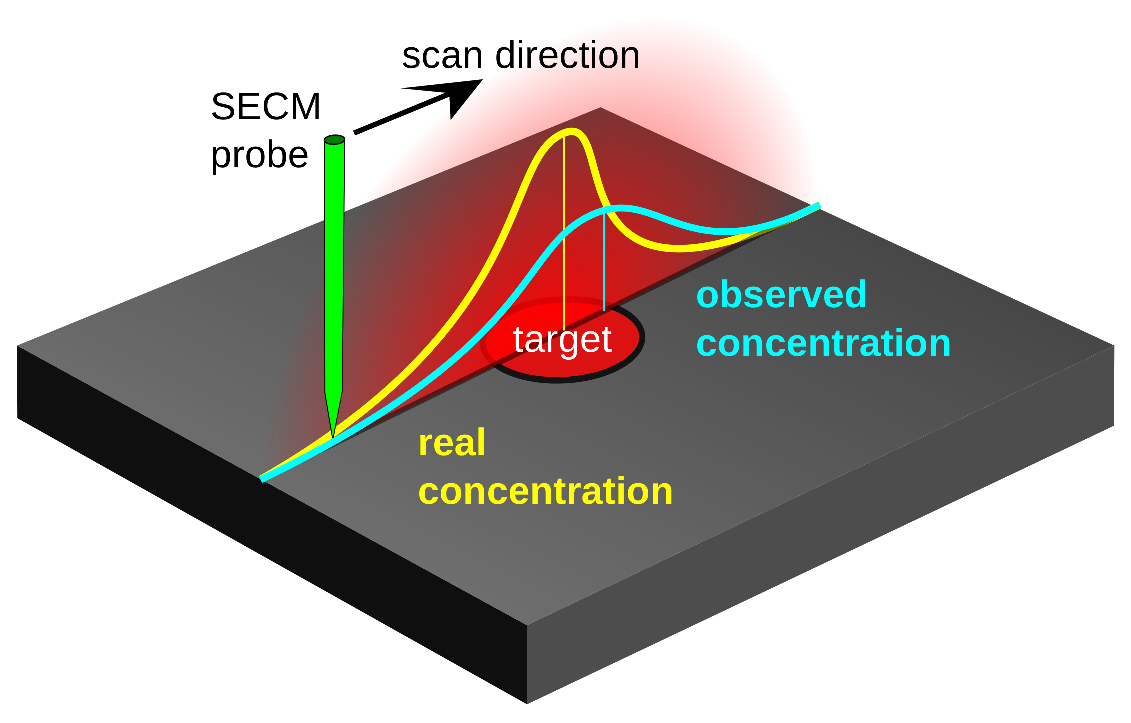
\includegraphics[width=0.8\textwidth]{distortion2.eps}
\end{frame}

\begin{frame}
	\frametitle{Why is it so important to complete the scan quickly?}
	\framesubtitle{Example: corrosion of a magnesium alloy}
	\includegraphics[width=1\textwidth]{timelapse.eps}\\
\centering
Corrosion of the AZ63 magnesium-aluminium-zinc alloy.
%Location of the anodic and cathodic spots change quickly. High-speed scanning is required to complete the scan before the studied system changes.
\end{frame} 

\begin{frame}
\frametitle{Trade-off triangle of potentiometric SECM}
\begin{center}
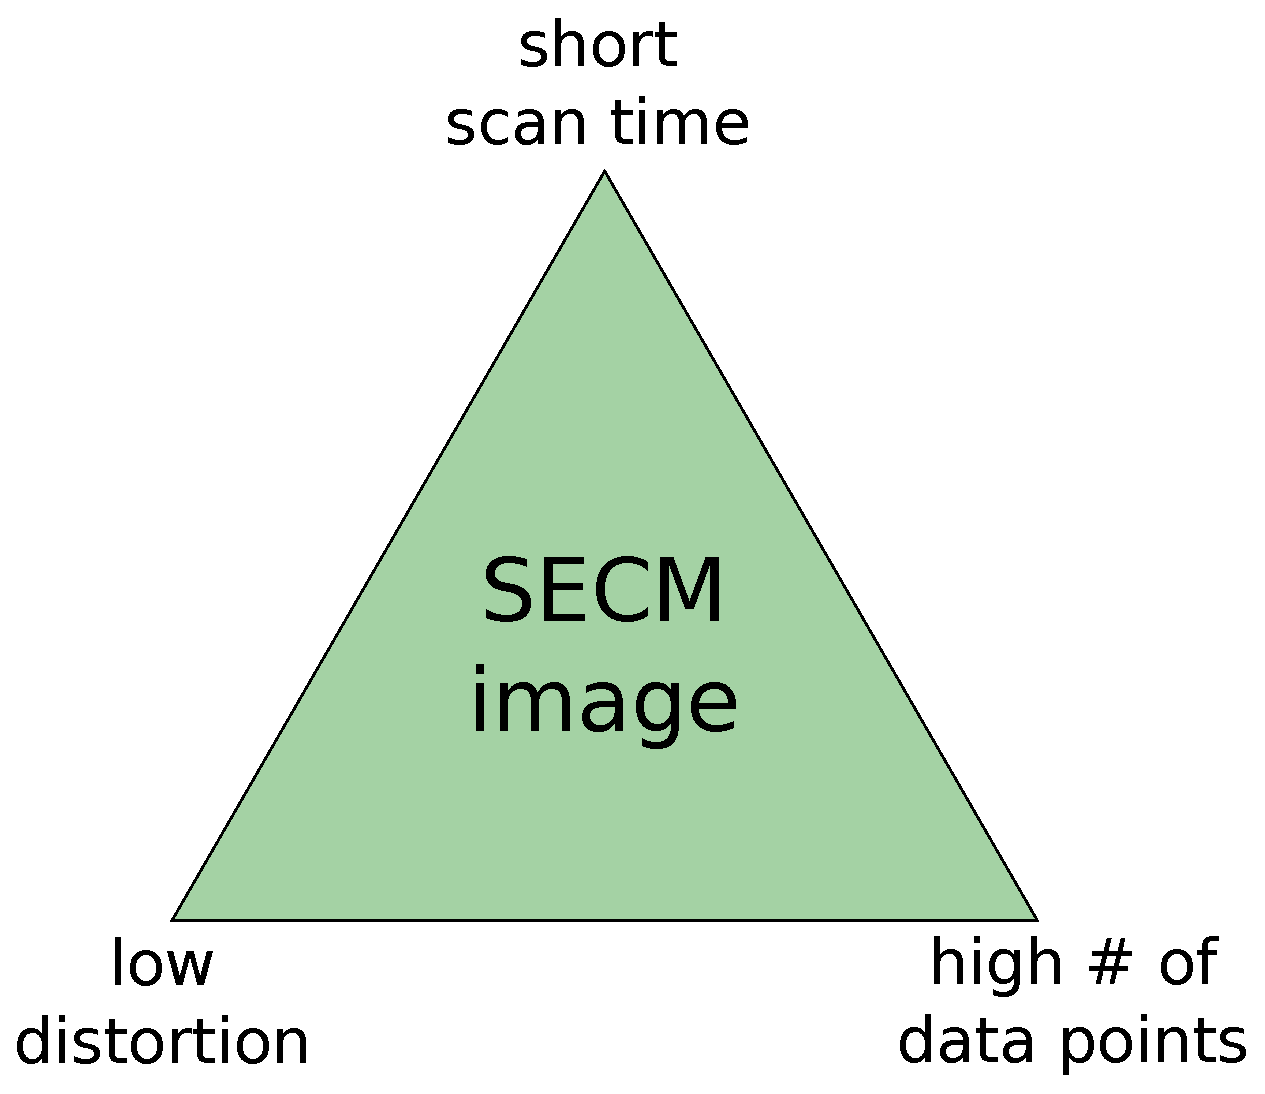
\includegraphics[width=0.5\textwidth]{trade-off.eps}
\end{center}
\end{frame}

\begin{frame}[plain]
\centering
Solution \#1:
Solid contact micropipettes as SECM probes.
\end{frame}

\begin{frame}
\frametitle{Liquid vs. solid contact micropipettes}
\framesubtitle{Comparison of construction}
\begin{center}
\quad\quad\quad\quad Liquid contact \hfill Solid contact \quad\quad\quad\quad

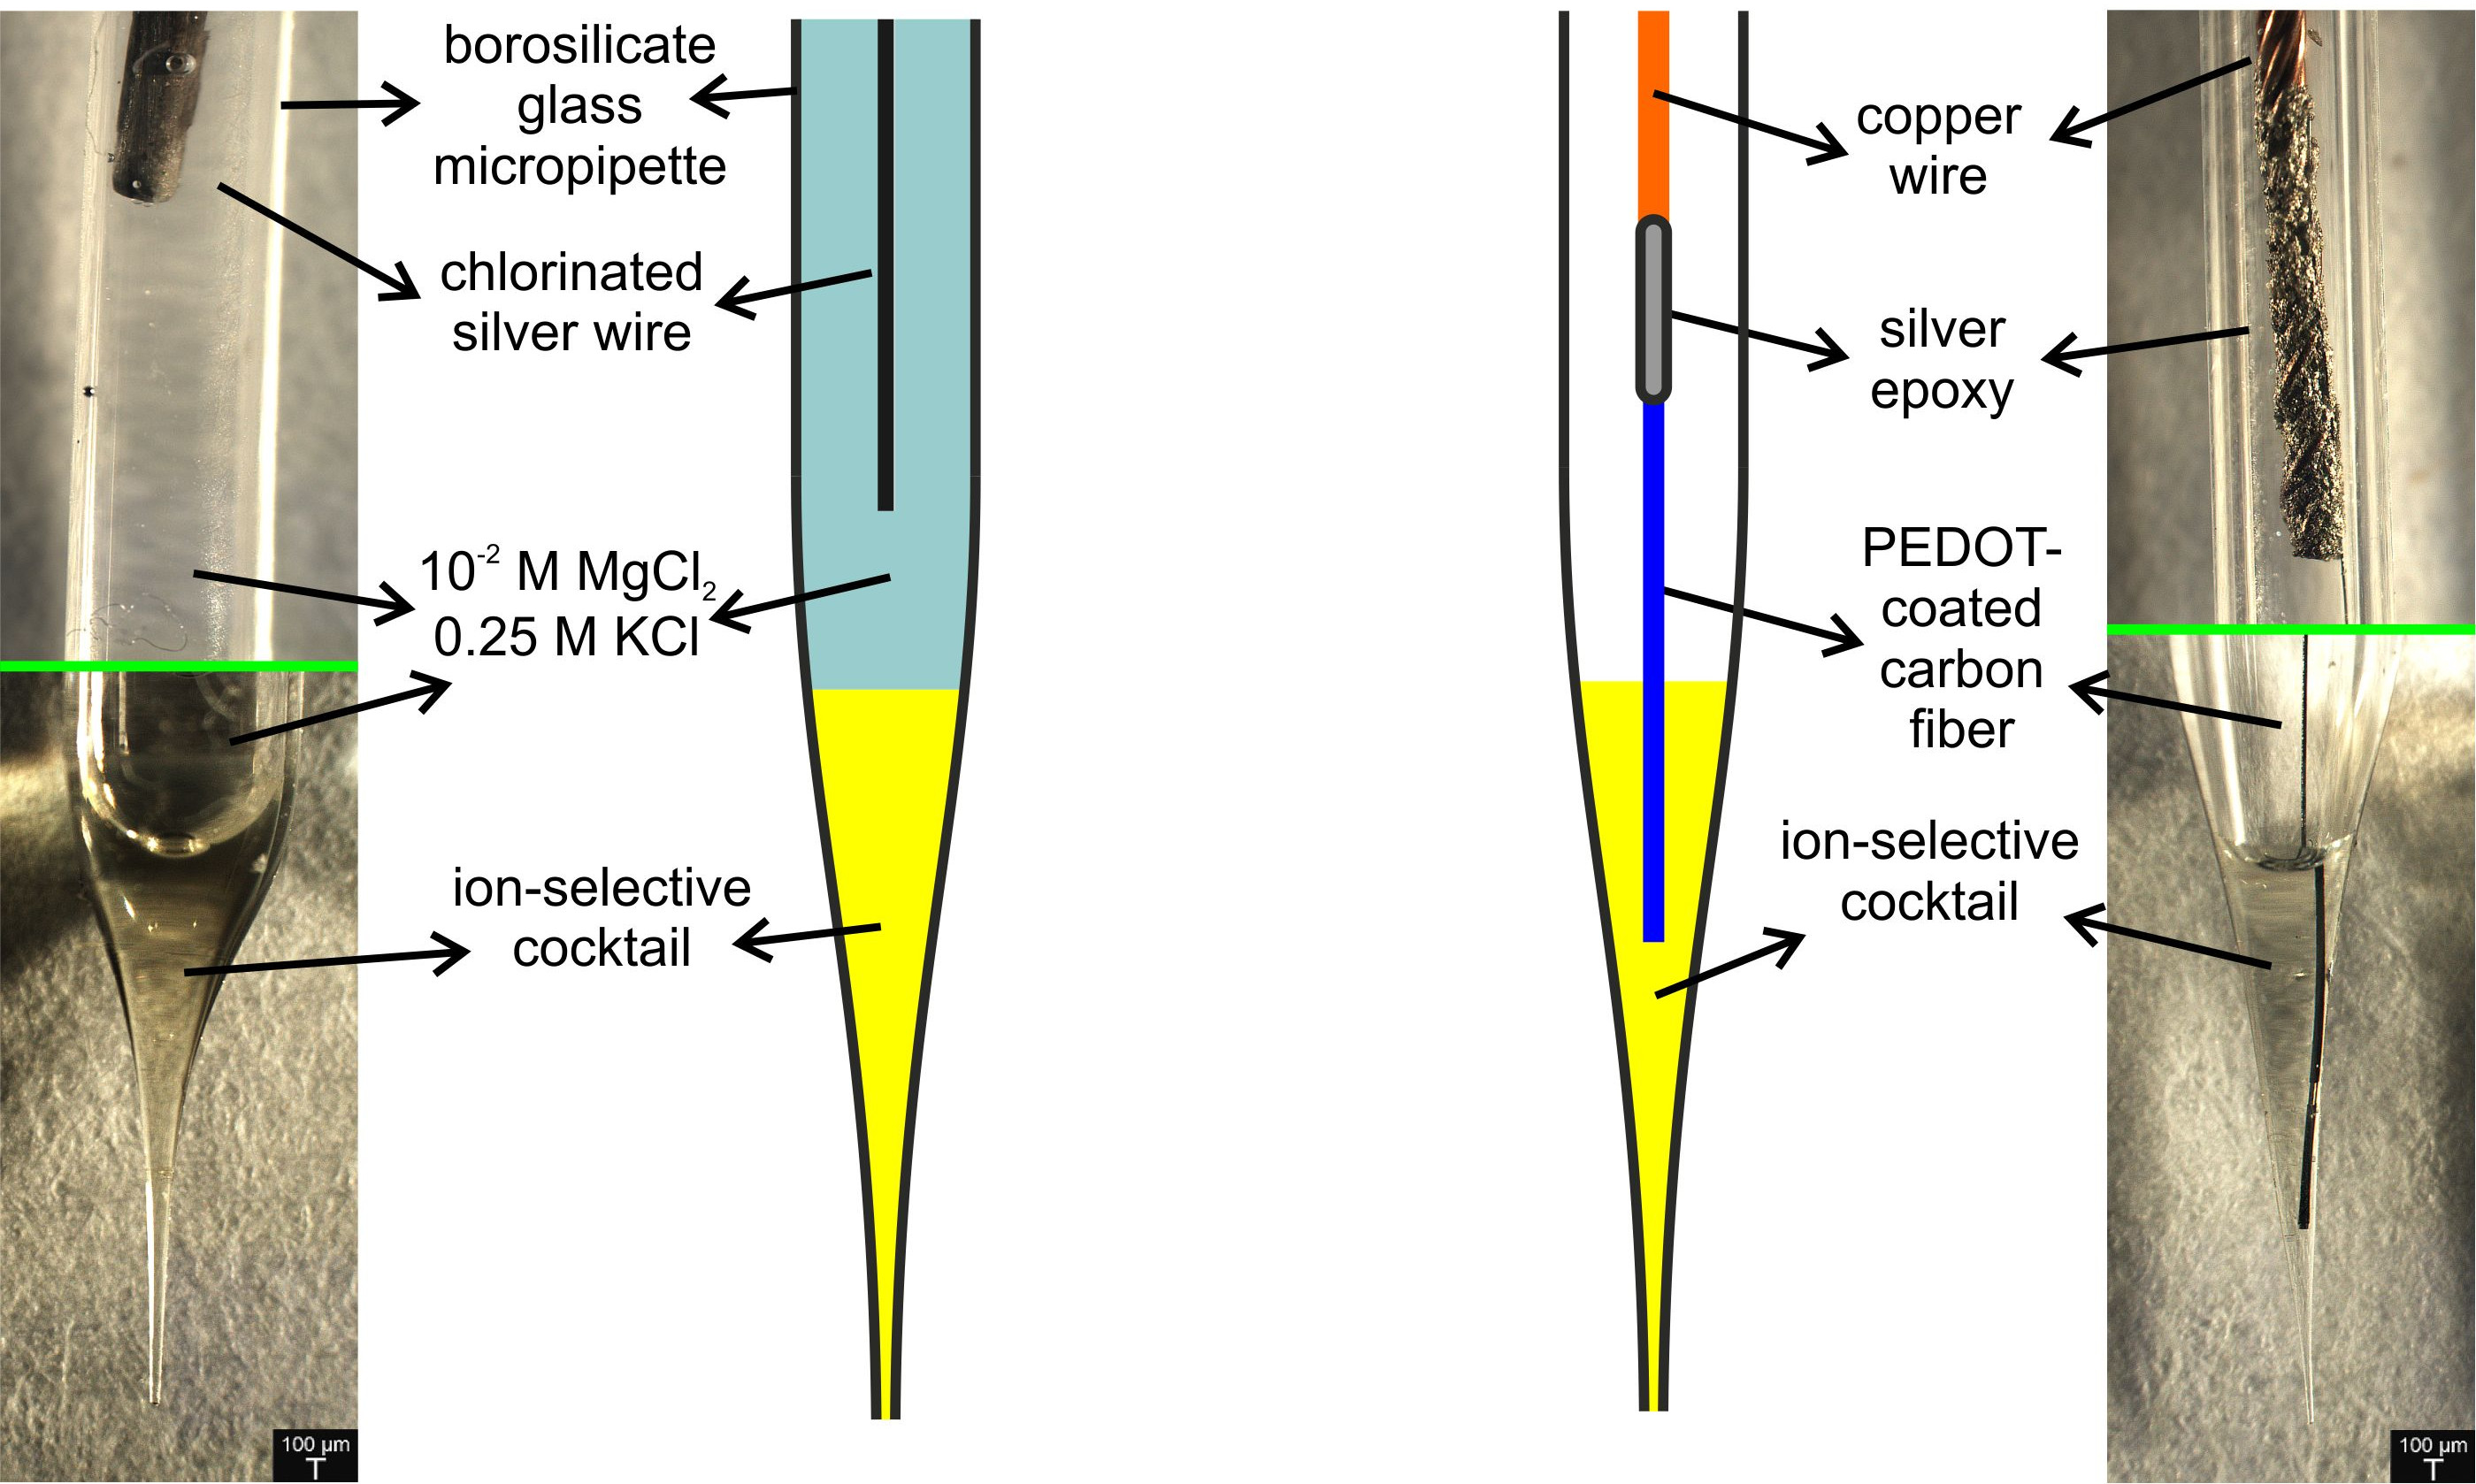
\includegraphics[width=0.9\textwidth]{liquid_solid.jpg}
\end{center}
\end{frame}

\begin{frame}
\frametitle{Comparison of the electrodes' resistance}
\framesubtitle{Experimental setup and result}
\begin{center}
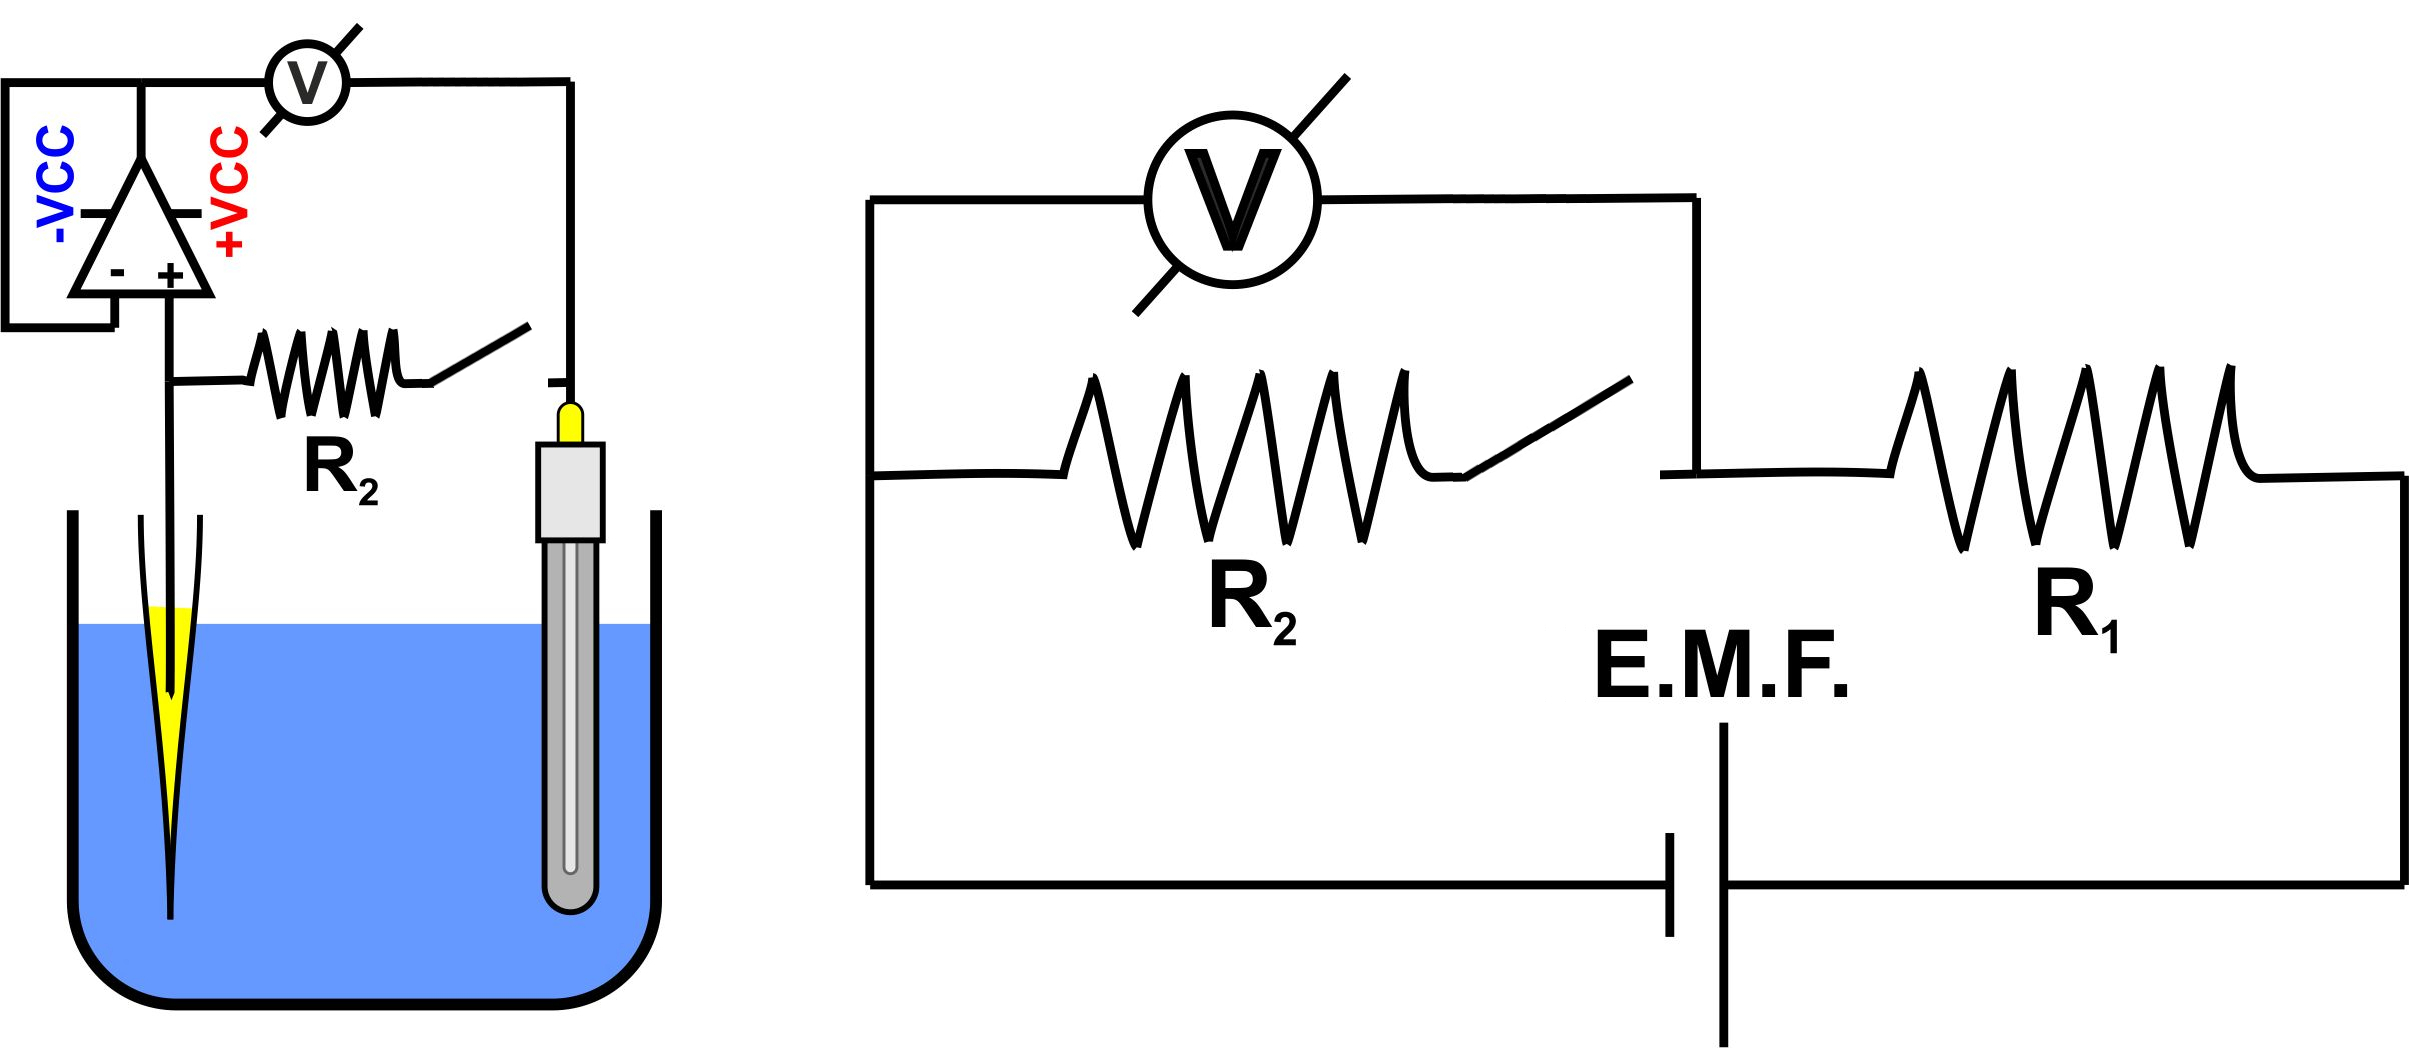
\includegraphics[width=0.7\textwidth]{divider_switch.jpg}
\vfill
\begin{table}
                \centering
                \begin{tabular}{r c}
                        %\hline
                        Type & R$_{ISME}$ / G$\ohm$ \\
			\cline{1-2}
			Liquid contact & \textbf{\textcolor{white!100}{\colorbox{red!100}{4.80}}} \\
                        Solid contact &  \textbf{\textcolor{black!100}{\colorbox{green!100}{0.56}}} \\

                \end{tabular}
\end{table}
\end{center}
\end{frame}

\begin{frame}
\frametitle{Comparison of the electrodes' performance}
\framesubtitle{Experimental setup}
\begin{center}
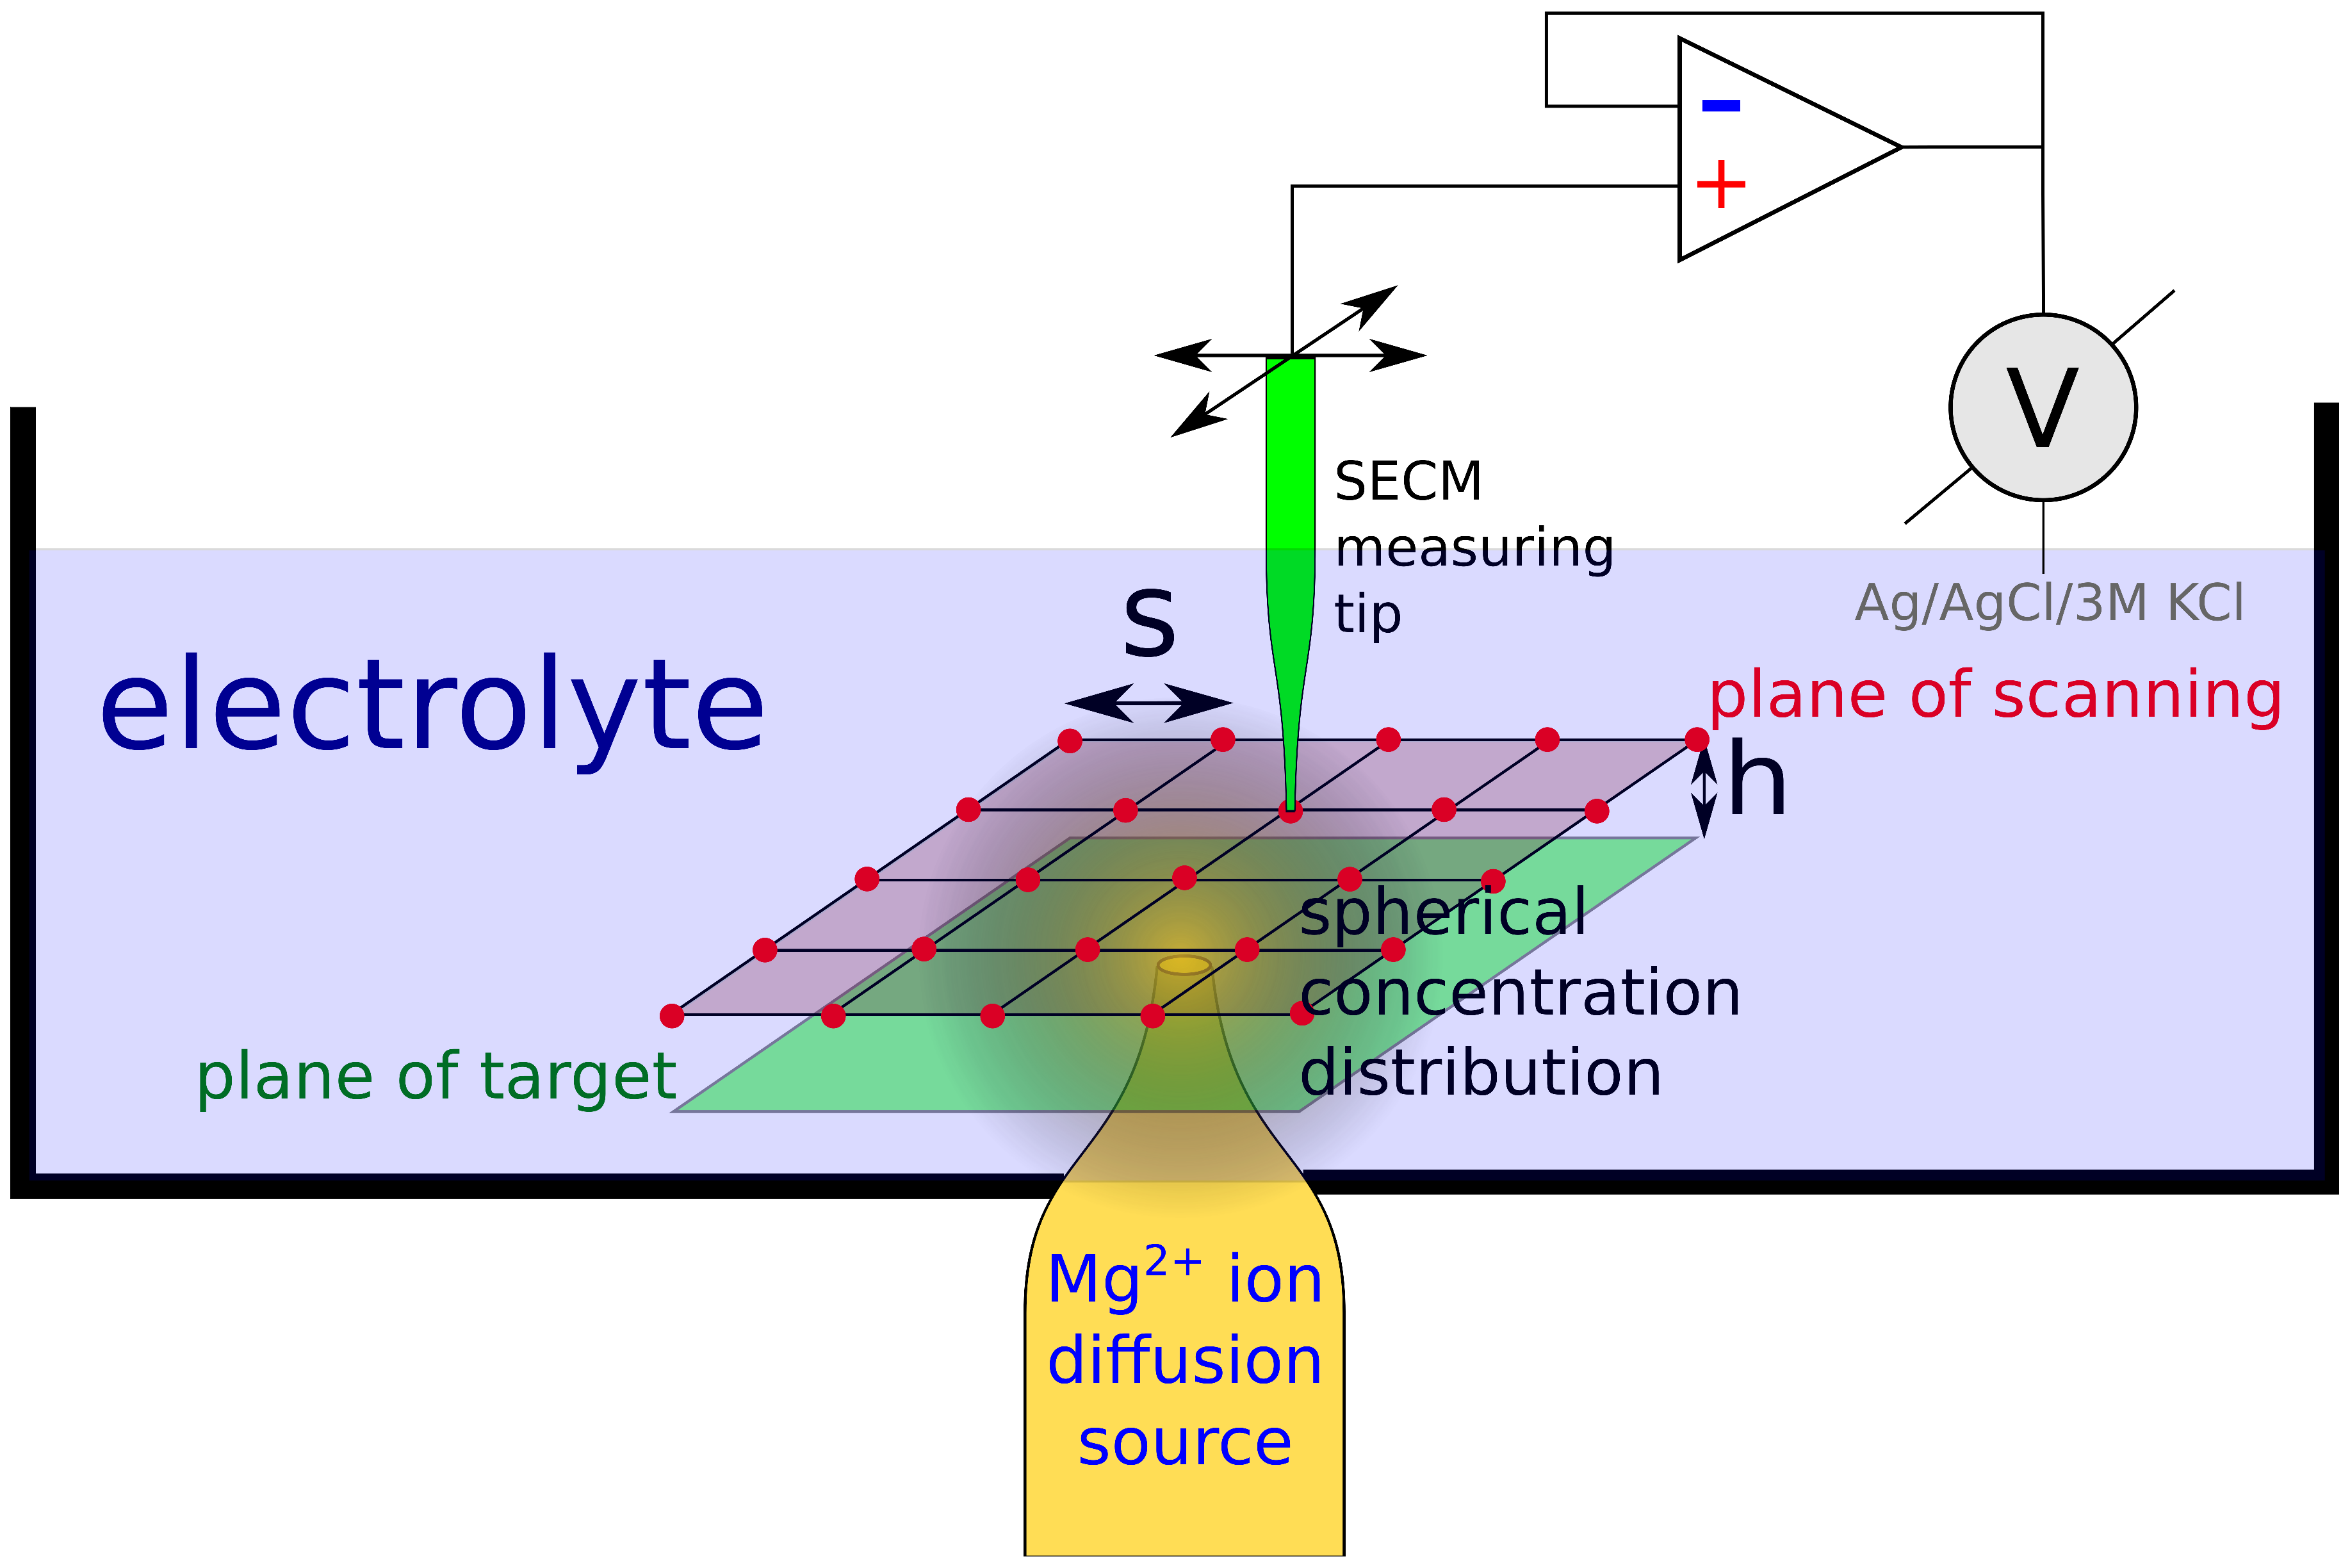
\includegraphics[width=0.9\textwidth]{setup.eps}
\end{center}
\end{frame}

\begin{frame}
	\frametitle{Comparison of the electrodes' performance} 
	\framesubtitle{Results}
	\centering
	\includegraphics[trim = 10mm 30mm 0mm 20mm, clip, width=0.4\textwidth, angle=-90]{liquid_Mg.eps}\hfill\includegraphics[trim = 10mm 30mm 0mm 20mm, clip, width=0.4\textwidth, angle=-90]{solid_Mg.eps}
\end{frame}

\begin{frame}
\frametitle{Application in corrosion science: galvanic corrosion of Mg}
\framesubtitle{Experimental setup}
\begin{center}
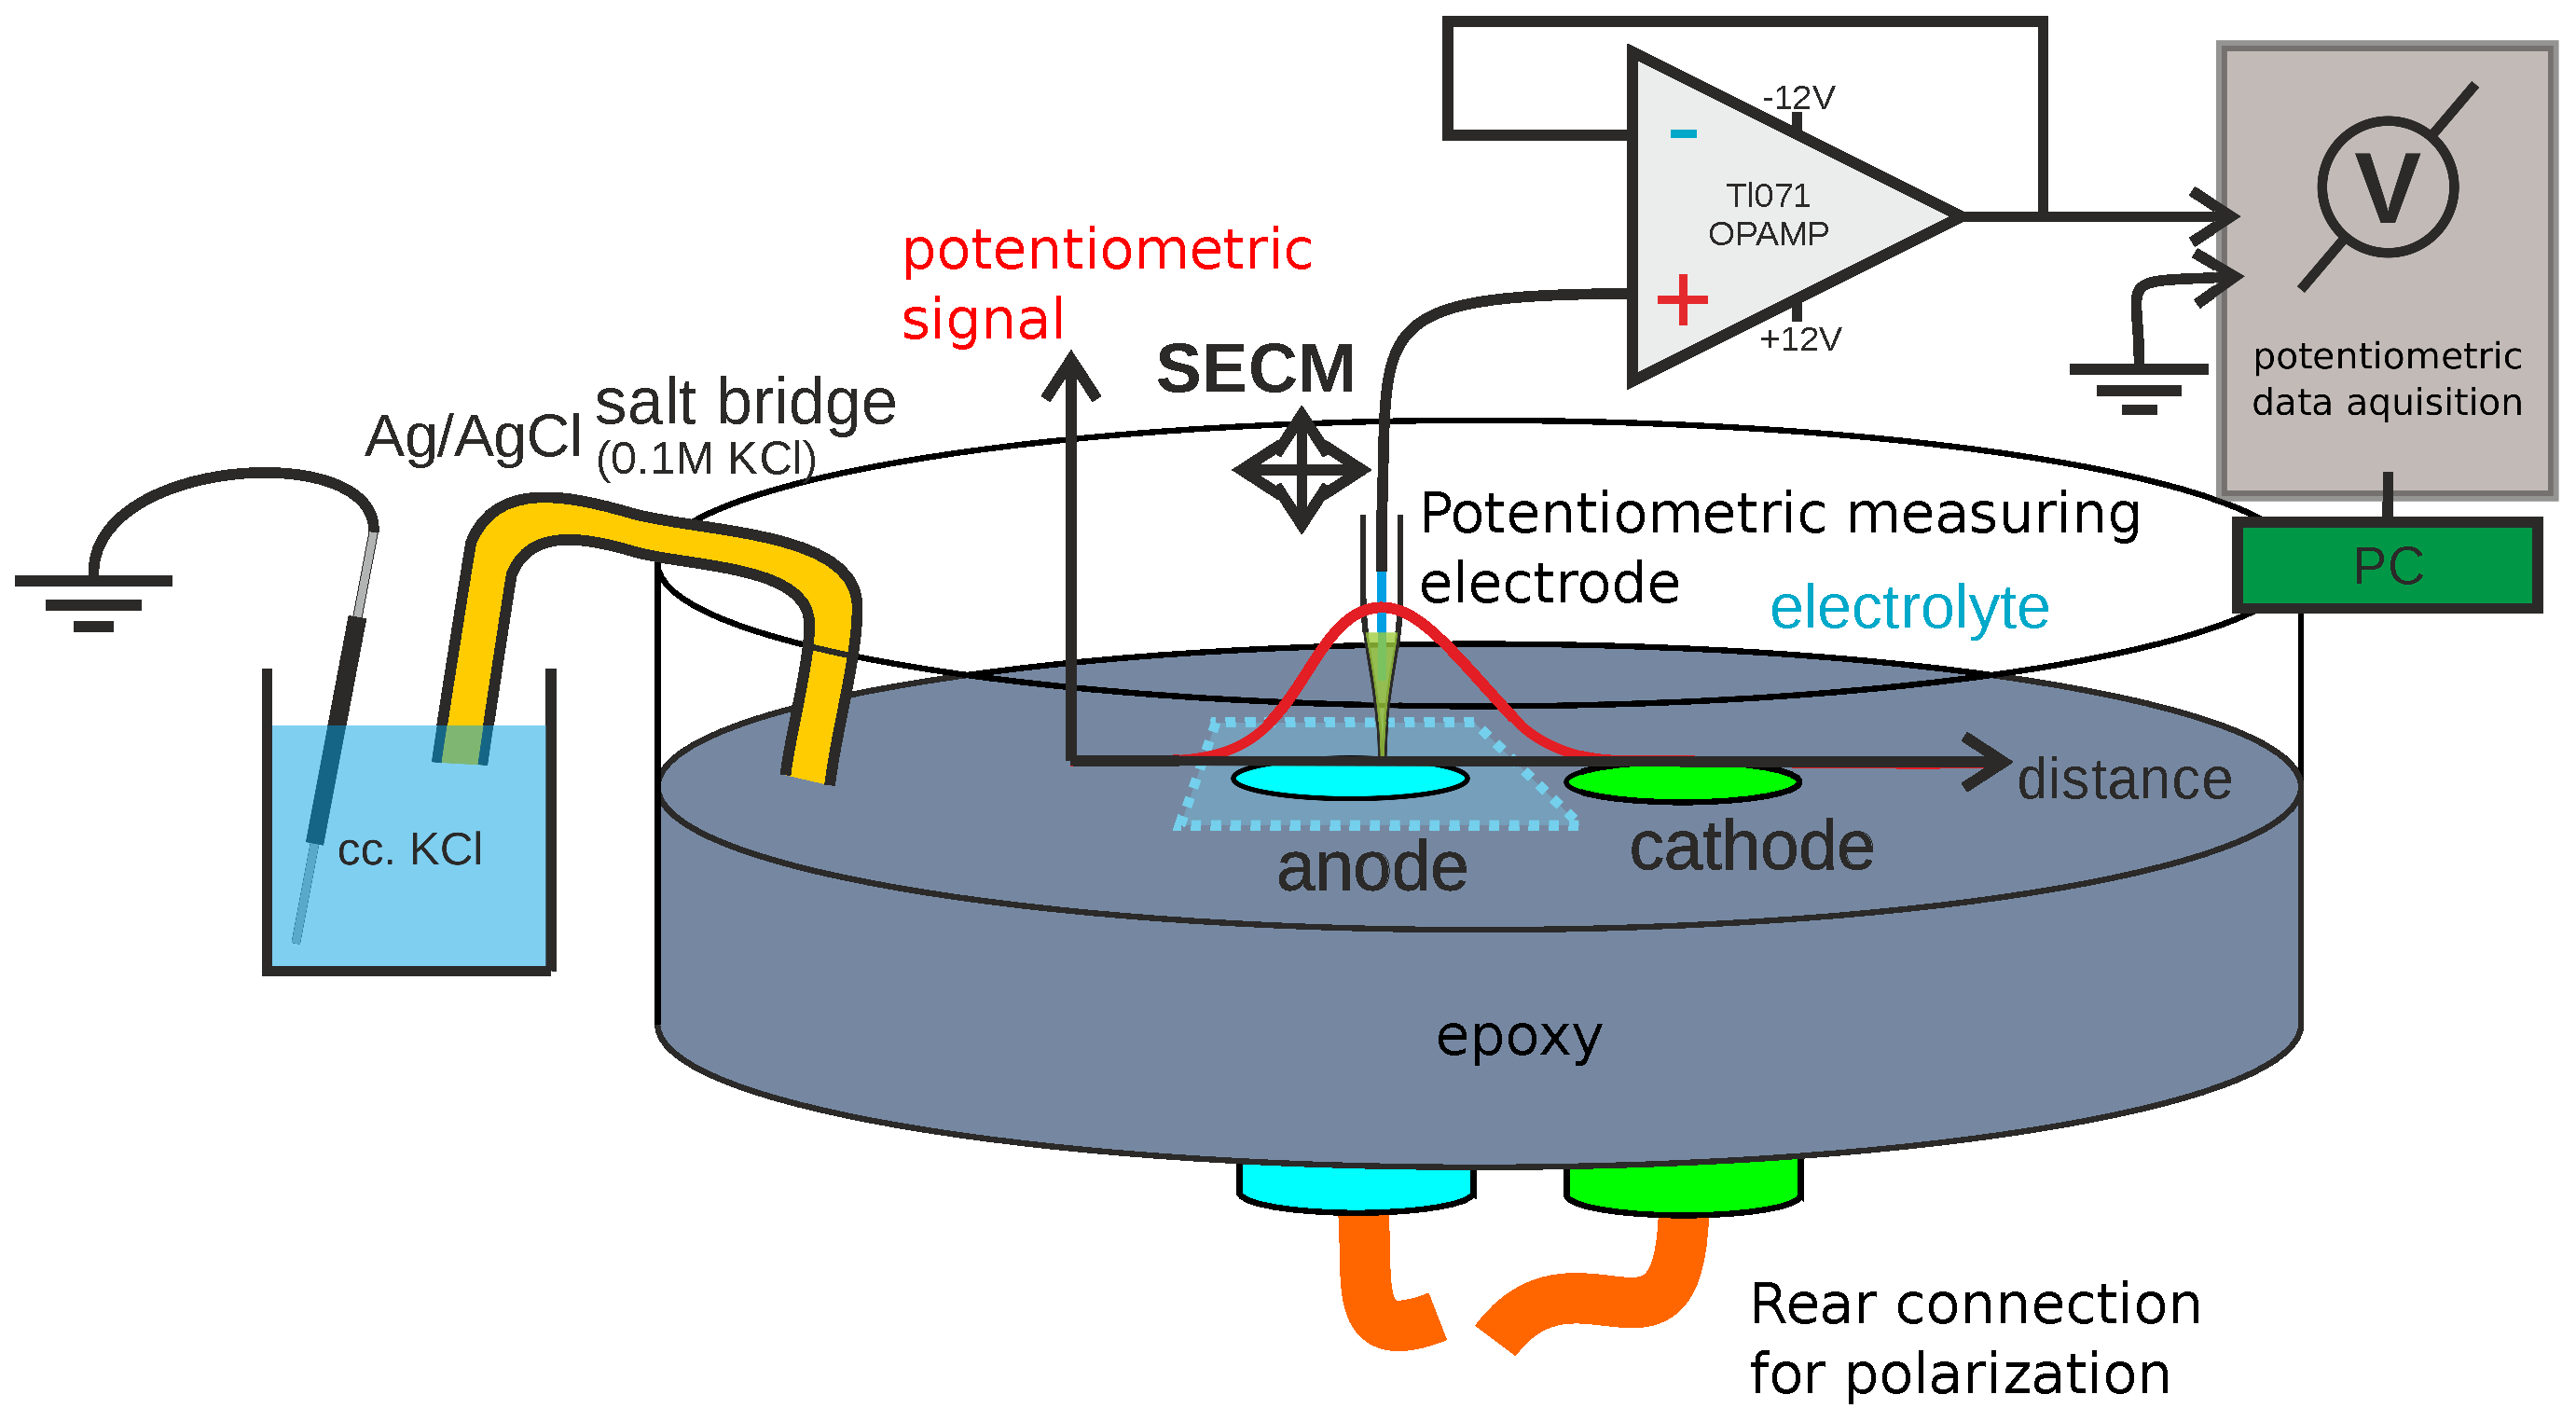
\includegraphics[width=0.9\textwidth]{model.eps}
\end{center}
\end{frame}

\begin{frame}
	\frametitle{Application in corrosion science: galvanic corrosion of Mg} 
	\framesubtitle{Results}
	\centering
	\quad\quad\quad\quad Liquid contact \hfill Solid contact \quad\quad\quad\quad\quad

	\includegraphics[trim = 10mm 30mm 0mm 20mm, clip, width=0.4\textwidth, angle=-90]{liquid_coupled.eps}\includegraphics[trim = 10mm 30mm 0mm 20mm, clip, width=0.4\textwidth, angle=-90]{solid_coupled.eps}
\end{frame}



\begin{frame}[plain]
\centering
Solution \#2:
Optimizing scanning patterns and algorithms.
\end{frame}

\begin{frame}
	\frametitle{"Traditional" scanning algorithms for the 2D raster pattern}
	\framesubtitle{1. "Meander" and "fast comb" scanning algorithms}
	\includegraphics[width=0.3\textwidth, angle=-90]{meander_pattern.eps}\includegraphics[width=0.3\textwidth, angle=-90]{meander_sim.eps}\\
		\includegraphics[width=0.3\textwidth, angle=-90]{fastcomb_pattern.eps}\includegraphics[width=0.3\textwidth, angle=-90]{fastcomb_sim.eps}
	\vfill
\end{frame}

\begin{frame}
	\frametitle{"Traditional" scanning algorithms for the 2D raster pattern}
	\framesubtitle{2. "Comb" scanning algorithm}
	\includegraphics[width=0.3\textwidth, angle=-90]{comb_pattern.eps}\includegraphics[width=0.3\textwidth, angle=-90]{comb_sim.eps}
	\vfill
\end{frame}



\begin{frame}
	\frametitle{The RC time constant} 
	\centering
	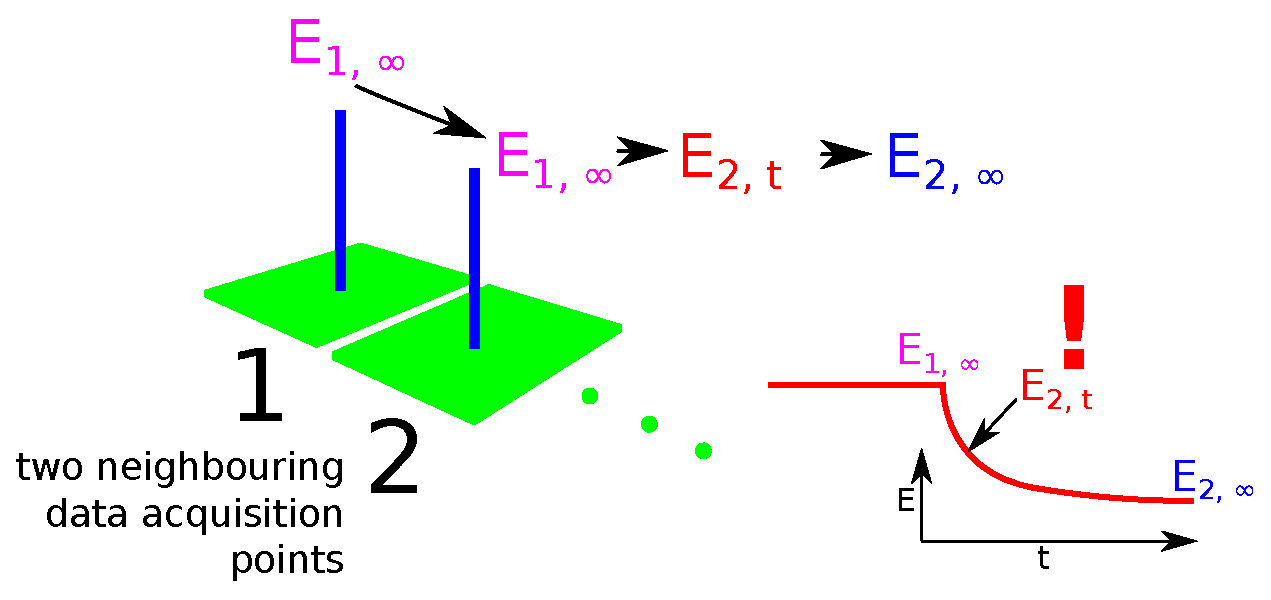
\includegraphics[width=1\textwidth]{t.eps}
\end{frame}



\begin{frame}
	\frametitle{New SECM scanning patterns based on the polar-coordinate system}
	\centering	
	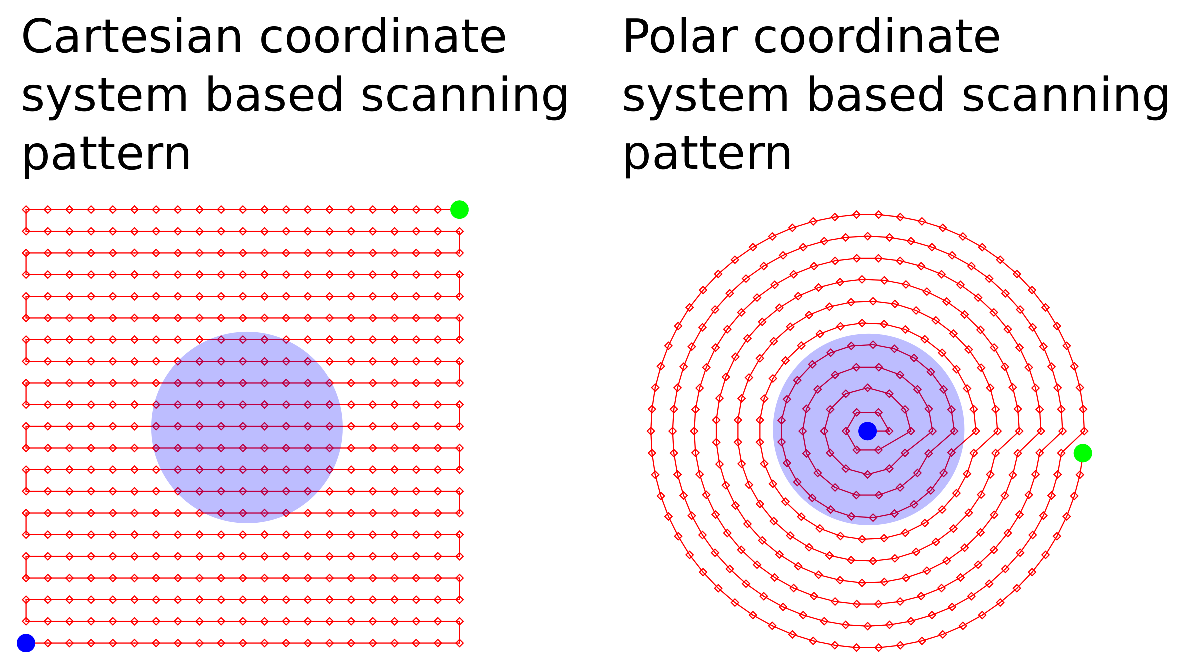
\includegraphics[width=0.7\textwidth]{cartesian_vs_polar.eps}
	
	\vfill
\end{frame}



\begin{frame}
	\frametitle{New SECM scanning patterns based on the polar-coordinate system}	
	\framesubtitle{Simulated scans with the "web" and the "arc" algorithms}
	\includegraphics[width=0.3\textwidth, angle=-90]{web_pattern.eps}\includegraphics[width=0.3\textwidth, angle=-90]{web_sim.eps}\\
		\includegraphics[width=0.3\textwidth, angle=-90]{arc_pattern.eps}\includegraphics[width=0.3\textwidth, angle=-90]{arc_sim.eps}
	\vfill
\end{frame}


\begin{frame}
	\frametitle{Comparison of the simulated scans}
Parameters of the simulations:\\
\begin{itemize}
\item 2000 $\upmu$m $\times$ 2000 $\upmu$m scan area,
\item 100 $\upmu$m $\times$ 100 $\upmu$m resolution,
\item 1 s for each data aquisition point,
\item 500 $\upmu$m/s probe positioning speed.
\end{itemize}

\vfill
\begin{table}
		\label{table:comp}
		\centering
		\begin{tabular}{r c c c}
			Algorithm & \#n & time (s) & mean squared error \\
			\hline
			Meander & 441 & 440 & $2.75\times 10^{-2}$ \\
			Fast comb& 441 & 520  & $2.07\times 10^{-2}$ \\
			Comb & 441 & 881 & $2.75\times 10^{-2}$ \\
			Web & 110 & 109 & $9.63\times 10^{-3}$ \\
			Arc & 341 & 340 & $2.95\times 10^{-3}$ \\
		\end{tabular}
\end{table}
\end{frame}

\begin{frame}
	\frametitle{Confirmation with experimental SECM scans}
	\framesubtitle{Traditional scanning algorithms}
	\includegraphics[width=0.3\textwidth, angle=-90]{meander.eps}\includegraphics[width=0.3\textwidth, angle=-90]{fastcomb.eps}\\
	\includegraphics[width=0.3\textwidth, angle=-90]{comb.eps}
	\vfill
	Images recorded with the meander, fast comb, and comb algorithms.
\end{frame}

\begin{frame}
	\frametitle{Confirmation with experimental SECM scans}
	\framesubtitle{New scanning algorithms}
	\includegraphics[width=0.3\textwidth, angle=-90]{web.eps}\includegraphics[width=0.3\textwidth, angle=-90]{arc.eps}
	\vfill
	Images recorded with the web, and the arc algorithms.
	\vfill
	Scans are completed 75\% and 20\% faster, images have almost 10 times less distortion.
\end{frame}


\begin{frame}
	\frametitle{Example 1: SECM study on the effectiveness of corrosion protection coatings using the arc scanning pattern}
	\centering
	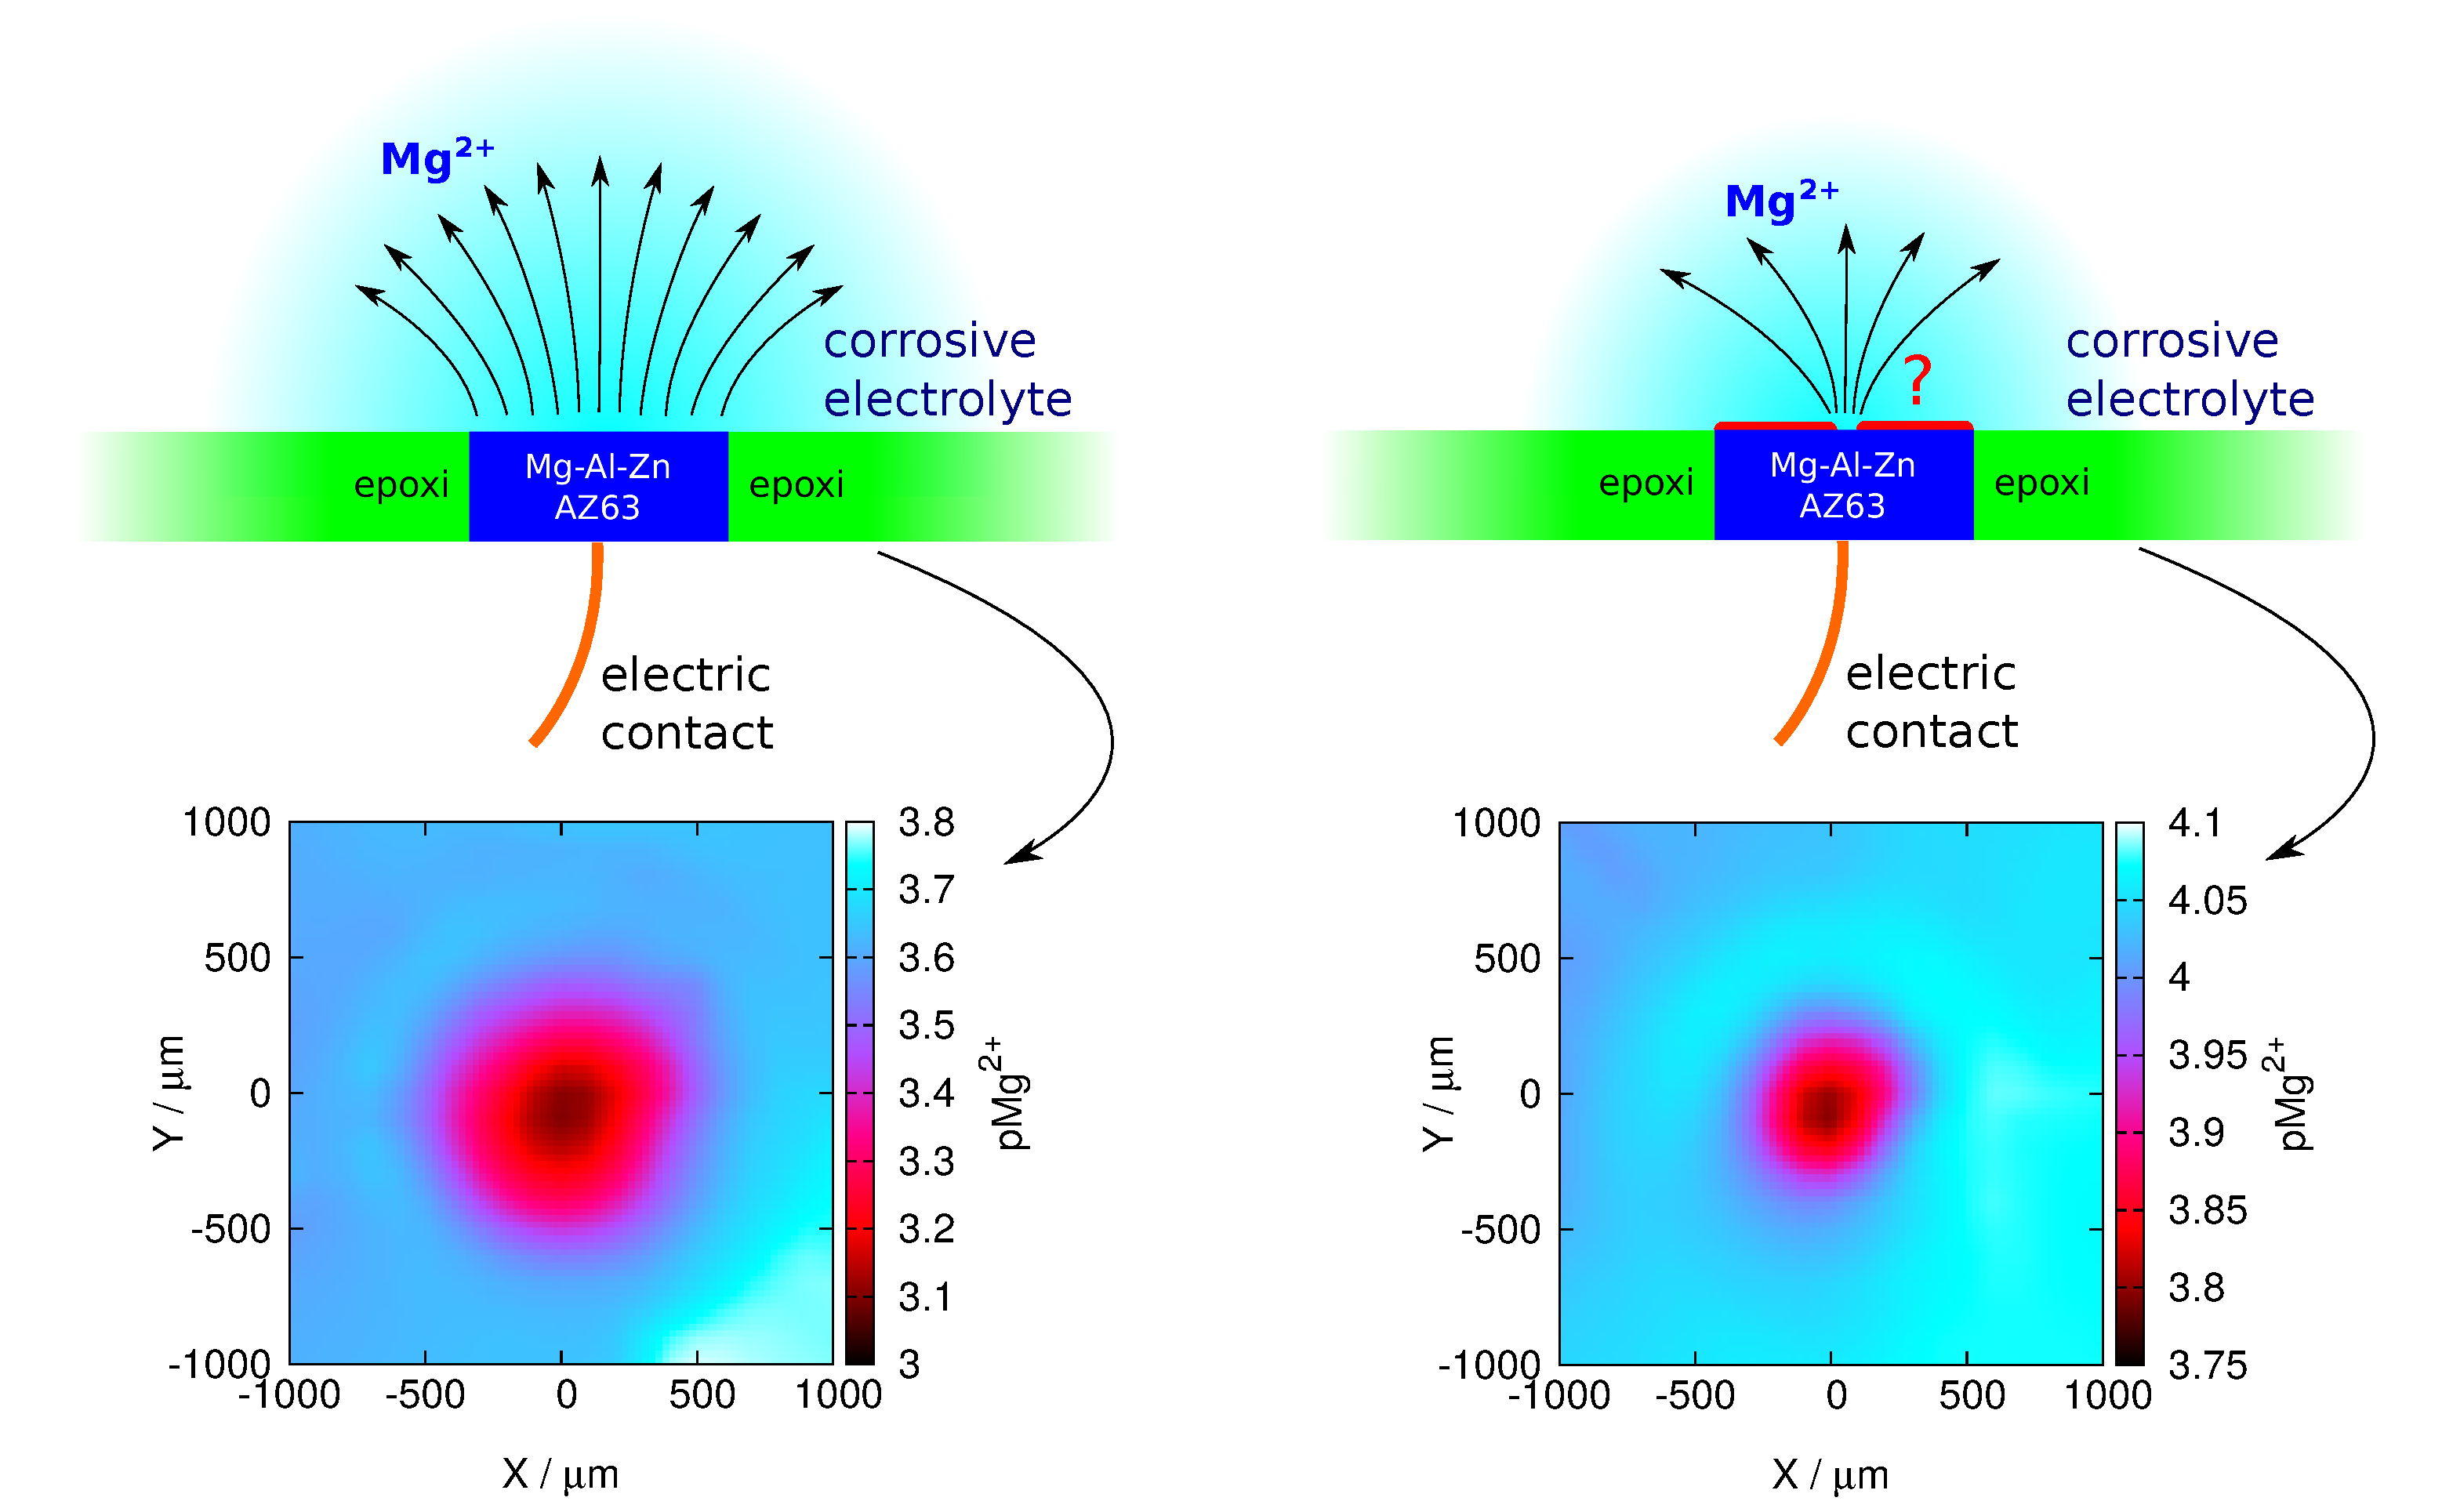
\includegraphics[width=1\textwidth]{nickel.eps}
\end{frame}

\begin{frame}
	\frametitle{Example 2: SECM study on the galvanic corrosion of the AZ63 alloy and iron, using the arc scanning pattern}
	\centering
	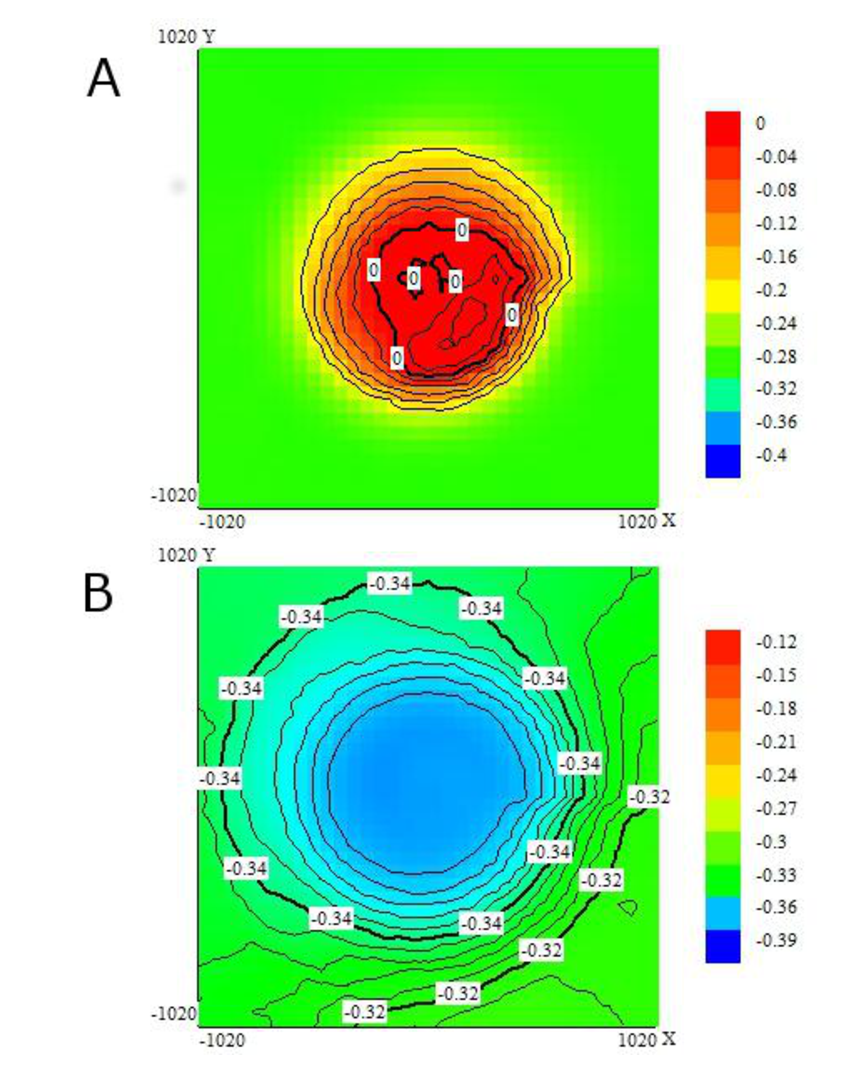
\includegraphics[width=0.4\textwidth]{galvanic.eps}
	
	pH-dependent potential map above the corroding (A) magnesium, and (B) iron samples.
\end{frame}



\begin{frame}
\centering
Solution \#2: Signal processing.
\end{frame}

\begin{frame}
\frametitle{Deconvolution of the distorted image}
\centering	
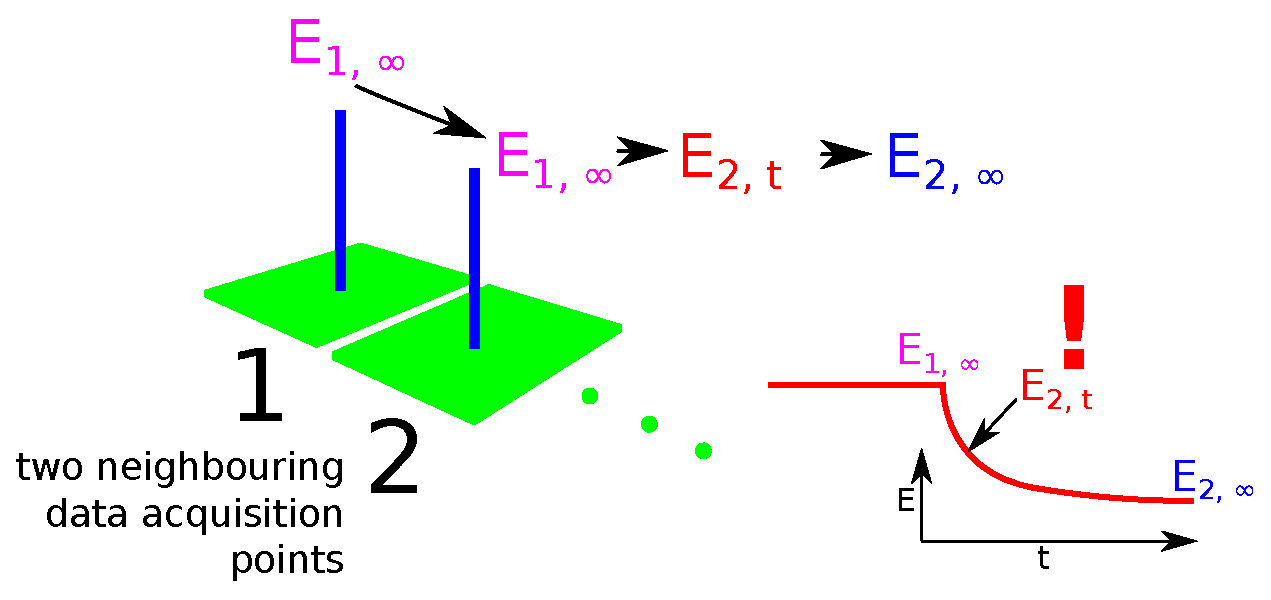
\includegraphics[width=0.8\textwidth]{t.eps}\\
\vfill
$E_{cell}(t) = E_{cell}(\infty) + [E_{cell}(0) - E_{cell}(\infty)]e^{-t/RC}$\\
\vfill
$E_{cell}(\infty)	= \frac {\displaystyle [E_{cell}(t) - E_{cell}(0)]e^{-t/RC}}	{\displaystyle 1 - e^{-t/RC}}$
\end{frame}


\begin{frame}
\begin{figure}
\begin{center}
\includegraphics[width=0.3\textwidth, angle=-90]{transient.eps}

\includegraphics[width=0.3\textwidth, angle=-90]{transient_cut.eps}
\end{center}
\vspace{0.5cm}

Response of an antimony/antimony-oxid - Ag/AgCl/3M KCl cell when pH changes from 4 to 6. RC time constant was determined from the fit.

%\caption{Transient response of the antimony microelectrode to analyte activity step. (A) The measuring and reference electrodes were dipped into buffer solutions with pH = 4 and pH = 6 respectively. (B) Response function fit (solid black line) on the section (red dots) of (A) from the pH step to the end of the curve when potential reaches equilibrium in the pH = 6 buffer.}
\label{fig:transient}
\end{figure}
\end{frame}


\begin{frame}
\frametitle{Minimal working example:}
\framesubtitle{Deconvolution of a response to activity step}
\begin{center}
\includegraphics[width=0.4\textwidth, angle=-90]{transient3.eps}
\end{center}

Transient response of the antimony microelectrode to analyte activity step (red), and deconvolutions performed with different $RC$ time-constants. The measured time-constant was $\tau = 3.76 s$ (cyan).
\end{frame}

\begin{frame}
\frametitle{Comparison of the deconvoluted time-potential recordings.}
\begin{table}
            %    \caption{Comparison of the deconvoluted time-potential recordings.}
                \label{table:rc}
                \centering
                \begin{tabular}{r c c c}
                        $e^{-0.5/RC}$ & $RC (s)$ & Mean squared error \\
                        \hline
                        raw recording (0) & raw recording (0) & 53.43 \\
                        0.7 & 1.4 & 22.03  \\
                        0.75 & 1.74 & 15.88  \\
                        0.8 & 2.24 & 9.01 \\
                        \textbf{0.8755} & \textbf{3.76} & \textbf{3.83} \\
                        0.9 & 4.75 & 16.99 \\
                        0.95 & 9.75 & 781.94 \\
                \end{tabular}
\end{table}
\end{frame}

%\begin{frame}
%\frametitle{SECM setup to test deconvolution}
%\begin{figure}
%\centering
%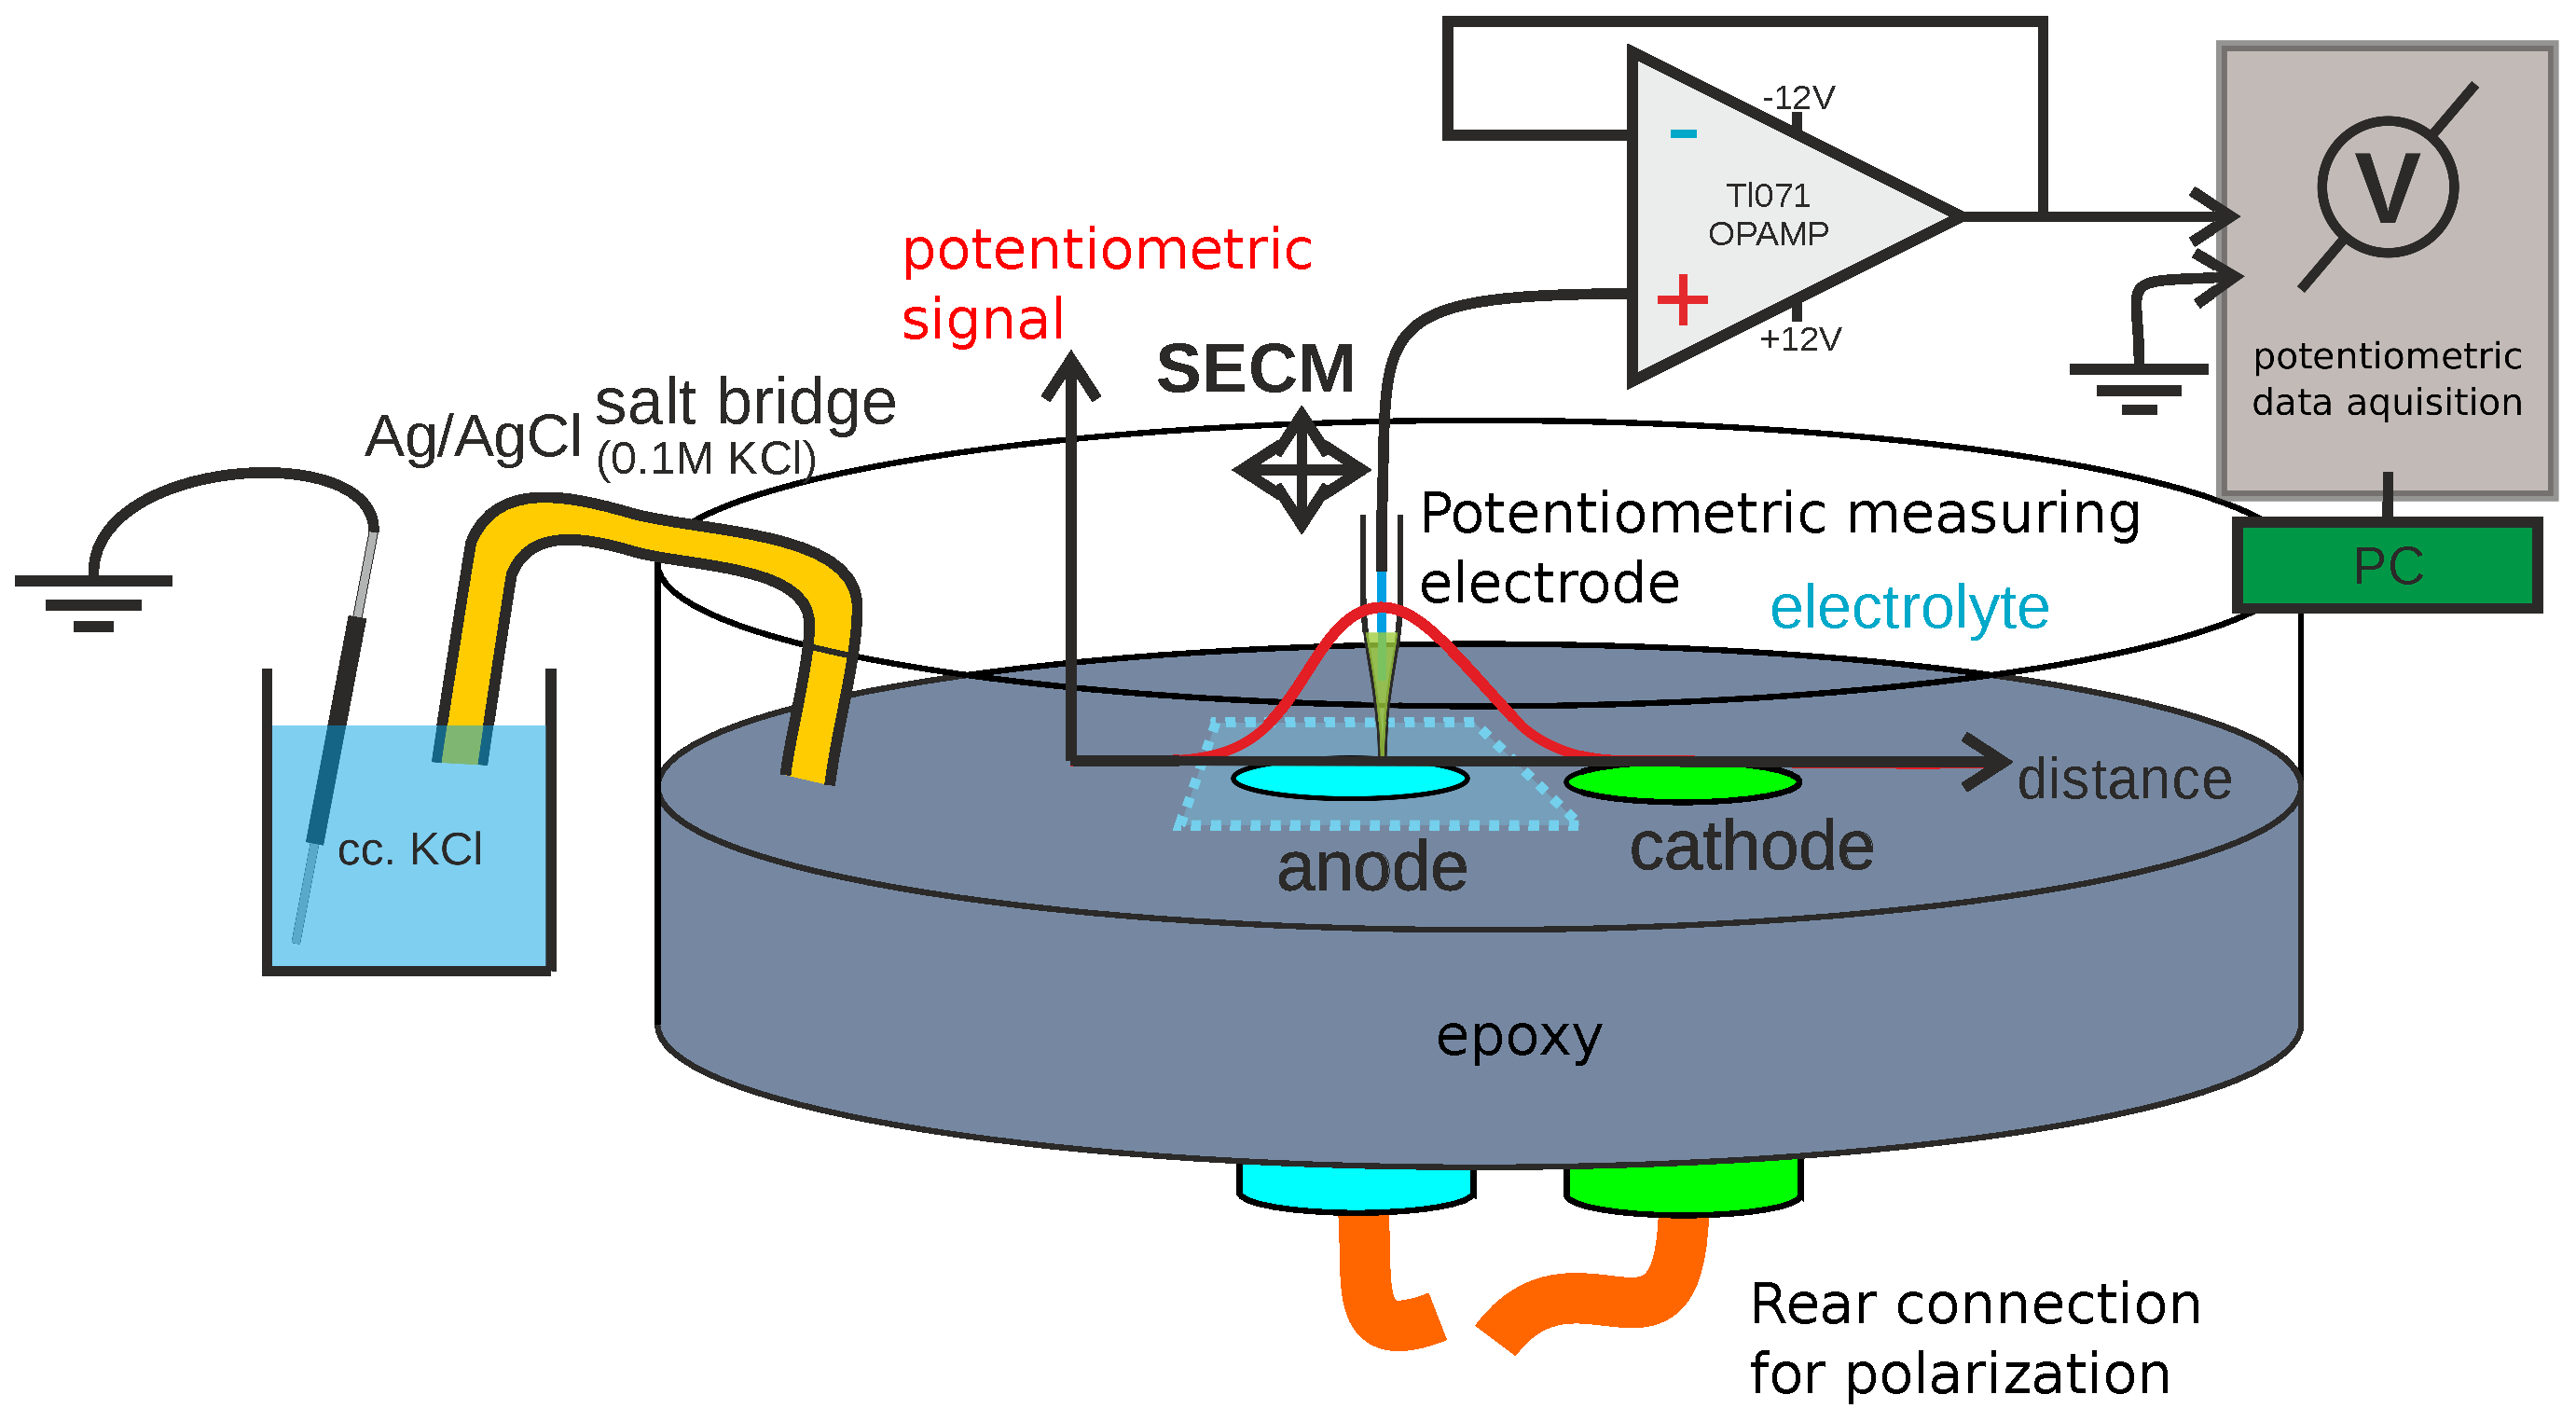
\includegraphics[width=0.8\textwidth]{model.eps}
%\caption{Sketch of the moulded model targets and the SECM scan setup used for these targets.}
%\end{figure}
%\end{frame}


\begin{frame}
\frametitle{One step further}
\framesubtitle{Deconvolution of linescans}
\begin{center}
% trim = top left bottom right
\includegraphics[trim = 0mm 0mm 0mm 0mm, clip, width=0.3\textwidth, angle=-90]{raw_lines_pH.eps}\includegraphics[trim = 0mm 0mm 0mm 0mm, clip, width=0.3\textwidth, angle=-90]{deconvoluted_lines_pH.eps}
%\includegraphics[trim = 0mm 0mm 0mm 0mm, clip, width=0.3\textwidth, angle=-90]{deconvoluted_lines8.eps}
\end{center}
(A) Raw, and, (B) deconvoluted SECM linescans above the center of the target, at h = 100 mm height, using three different equilibration periods: 0.5 s, (green), 1 s, (blue), and 5 s, (red).
\end{frame}


\begin{frame}
	\frametitle{Deconvolution of the distorted image}
	\framesubtitle{pH microscopy with antimony microelectrode}
	\includegraphics[width=0.3\textwidth, angle=-90]{13121313.eps}
	\includegraphics[width=0.3\textwidth, angle=-90]{13121313_deconvoluted.eps}\\
\end{frame}


%\begin{frame}
%	\frametitle{Deconvolution of the distorted image}
%	\includegraphics[width=0.3\textwidth, angle=-90]{13121313.eps}
%	\includegraphics[width=0.3\textwidth, angle=-90]{13121313_deconvoluted.eps}\\
%\end{frame}

%\begin{frame}
%	\centering
%	\includegraphics[width=0.8\textwidth]{polar_paper.eps}
%	\vfill	
%	\vfill
%	\includegraphics[width=0.8\textwidth]{deconvolution_paper.eps}
%\end{frame}

\begin{frame}
\begin{center}
\frametitle{Linescans with magnesium-ion selective micropipettes, and their deconvolution}
\includegraphics[width=0.3\textwidth]{mg.pdf}
\end{center}
\end{frame}


\begin{frame}
\begin{center}
\frametitle{2D scans with magnesium-ion selective micropipettes, and their deconvolution}
\includegraphics[width=0.6\textwidth]{mg_2d.pdf}
\end{center}
\end{frame}


\begin{frame}
	\frametitle{Example 3: SECM study on the galvanic corrosion of a zinc - copper galvanic pair}
	\framesubtitle{With antimony microelectrode}
\begin{figure}
\centering
%top left bottom right
\includegraphics[width=0.5\textwidth]{1.pdf}

\includegraphics[width=0.5\textwidth]{1_deconvoluted.pdf}

%\caption[Raw, and deconvoluted SECM image of a galvanically coupled zinc-copper pair.]{Raw (A), and deconvoluted (B) SECM image of a galvanically coupled zinc-copper pair. Left: zinc, right: copper. Diameter of the zinc and copper samples was 200 $\upmu$m. Corrosive electrolyte was 1 mM NaCl. Recorded $h$ = 100 $\upmu$m over the surface with a scanrate of 12.5 $\upmu$m/s.}
\end{figure}
\end{frame}

\begin{frame}
\frametitle{Example 4: Raw, and deconvoluted SECM image and microphoto of a corroding carbon-steel sample.}
\framesubtitle{With antimony microelectrode}
\begin{figure}
\centering
%top left bottom right
\includegraphics[trim = 10mm 30mm 0mm 10mm, clip, width=0.3\textwidth, angle=-90]{16012906.eps}\includegraphics[trim = 10mm 30mm 0mm 10mm, clip, width=0.3\textwidth, angle=-90]{16012906_deconvoluted.eps}

\includegraphics[width=0.24\textwidth]{cs_cut.jpg}

%\caption[Raw, and deconvoluted SECM image and microphoto of a corroding carbon-steel sample polarized anodically.]{Raw (A), and deconvoluted (B) SECM image and microphoto (C) of a corroding carbon-steel sample polarized anodically with a current density of 10 $mA/cm^2$. Measuring electrode was an antimony pH microelectrode. Potential was measured against an Ag/AgCl/3M KCl. Recorded $h$ = 100 $\upmu$m above the surface with probe movement speed of 1000 $\upmu$m/s, equilibration interval 0.4 s.}
\end{figure}
\end{frame}



\begin{frame}
	\frametitle{Summary}
\begin{itemize}
	\item Compromise between image quality and scan time in potentoimetric SECM.
	\item I've demonstrated two approaches to alleviate this compromise.
	\item With optimized scanning patterns and algorithms, scans are faster up to 4 times, imaging distortion is 10 times less.
	\item These algorithms work only with radially symmetric targets.
	\item Another approach is to deconvolution. Can be applied to any system. Image quality is drastically improved, and scan time is shorter.
\end{itemize}
\end{frame}

%\begin{frame}
%	\frametitle{Acknowledgements}


%This research was supported by the European Union and the State of Hungary, co-financed by the European Social Fund in the framework of T\'{A}MOP-4.2.4.A/ 2-11/1-2012-0001 'National Excellence Program'.	

%\end{frame}



\begin{frame}
\includegraphics[width=1\textwidth]{pecs.eps}
\end{frame}

\end{document}
